\documentclass[10pt,handout]{beamer}
\usetheme{Rochester}
\usepackage[utf8]{inputenc}
\usepackage{amsmath}
\usepackage{amsfonts}
\usepackage{amssymb}
%\setbeamertemplate{frametitle}[default][center]
\setbeamercolor{page number in head/foot}{fg=black}
\setbeamerfont{page number in head/foot}{size=\small}

\setbeamertemplate{footline}[page number]
%\beamertemplatenavigationsymbolsempty
%\setbeamertemplate{footline}[page number]
%\setbeamertemplate{footline}[frame number]
%\usepackage{siunitx}
\author{Justin Anguiano}
\title{MC Matching and Event Composition for Soft Muons}


%\setbeamercovered{transparent} 
%\setbeamertemplate{navigation symbols}{} 
%\logo{} 
\institute{University of Kansas} 
\date{\today} 
%\subject{} 
\begin{document}

\begin{frame}
\titlepage
\end{frame}



\begin{frame}{Summary}

\begin{columns}
\begin{column}{0.5\textwidth}
 \\
\begin{itemize}
\item[1.] Finalized MC matching and defined labeling
\item[2.] Defined gen flavor for both muons/ non muons
\item[3.] Looked at the composition of several processes w.r.t labels and gen flavor
\end{itemize}

\end{column}
\begin{column}{0.5\textwidth}
%\includegraphics[scale=.3]{xyold.pdf}
\end{column}
\end{columns}
\end{frame}

\begin{frame}{Data Samples}
\center{\textbf{MINIAODSIM}:}\\
 \url{/DYJetsToLL_M-50_HT-70to100_TuneCP5_13TeV-madgraphMLM-pythia8/RunIIFall17MiniAODv2-PU2017_12Apr2018_94X_mc2017_realistic_v14-v1/MINIAODSIM}\\
\quad \quad \\\
 \url{/TTJets_DiLept_TuneCP5_13TeV-madgraphMLM-pythia8/RunIIAutumn18MiniAOD-102X_upgrade2018_realistic_v15-v1/MINIAODSIM}\\

\url{/QCD_Pt_600to800_TuneCP5_13TeV_pythia8/RunIIWinter19PFCalibMiniAOD-2018Conditions_105X_upgrade2018_realistic_v4-v1/MINIAODSIM}\\


\quad \quad \\
\quad \quad \\
\scriptsize
*all datasets have corresponding NANO child
\end{frame}
\begin{frame}{Matching Criteria}

\begin{itemize}
\item[*] $\Delta R < 0.2$
\item[*] $\Delta P_T^{rel} < 0.2$  ---------------------  $\frac{|p_T^{mc} - p_T^{reco}|}{p_T^{mc}}$
\item[*] Resolve ambiguities \quad  --------- Forbid two RECO objects to match to the same GEN object
\item[*] Resolve by Quality \quad ----------- Choose the lowest $\Delta R$ pair 

\end{itemize}

\end{frame}
\begin{frame}{ DY } 

\quad \quad \\
\begin{columns}
\begin{column}{0.5\textwidth}
No Cut
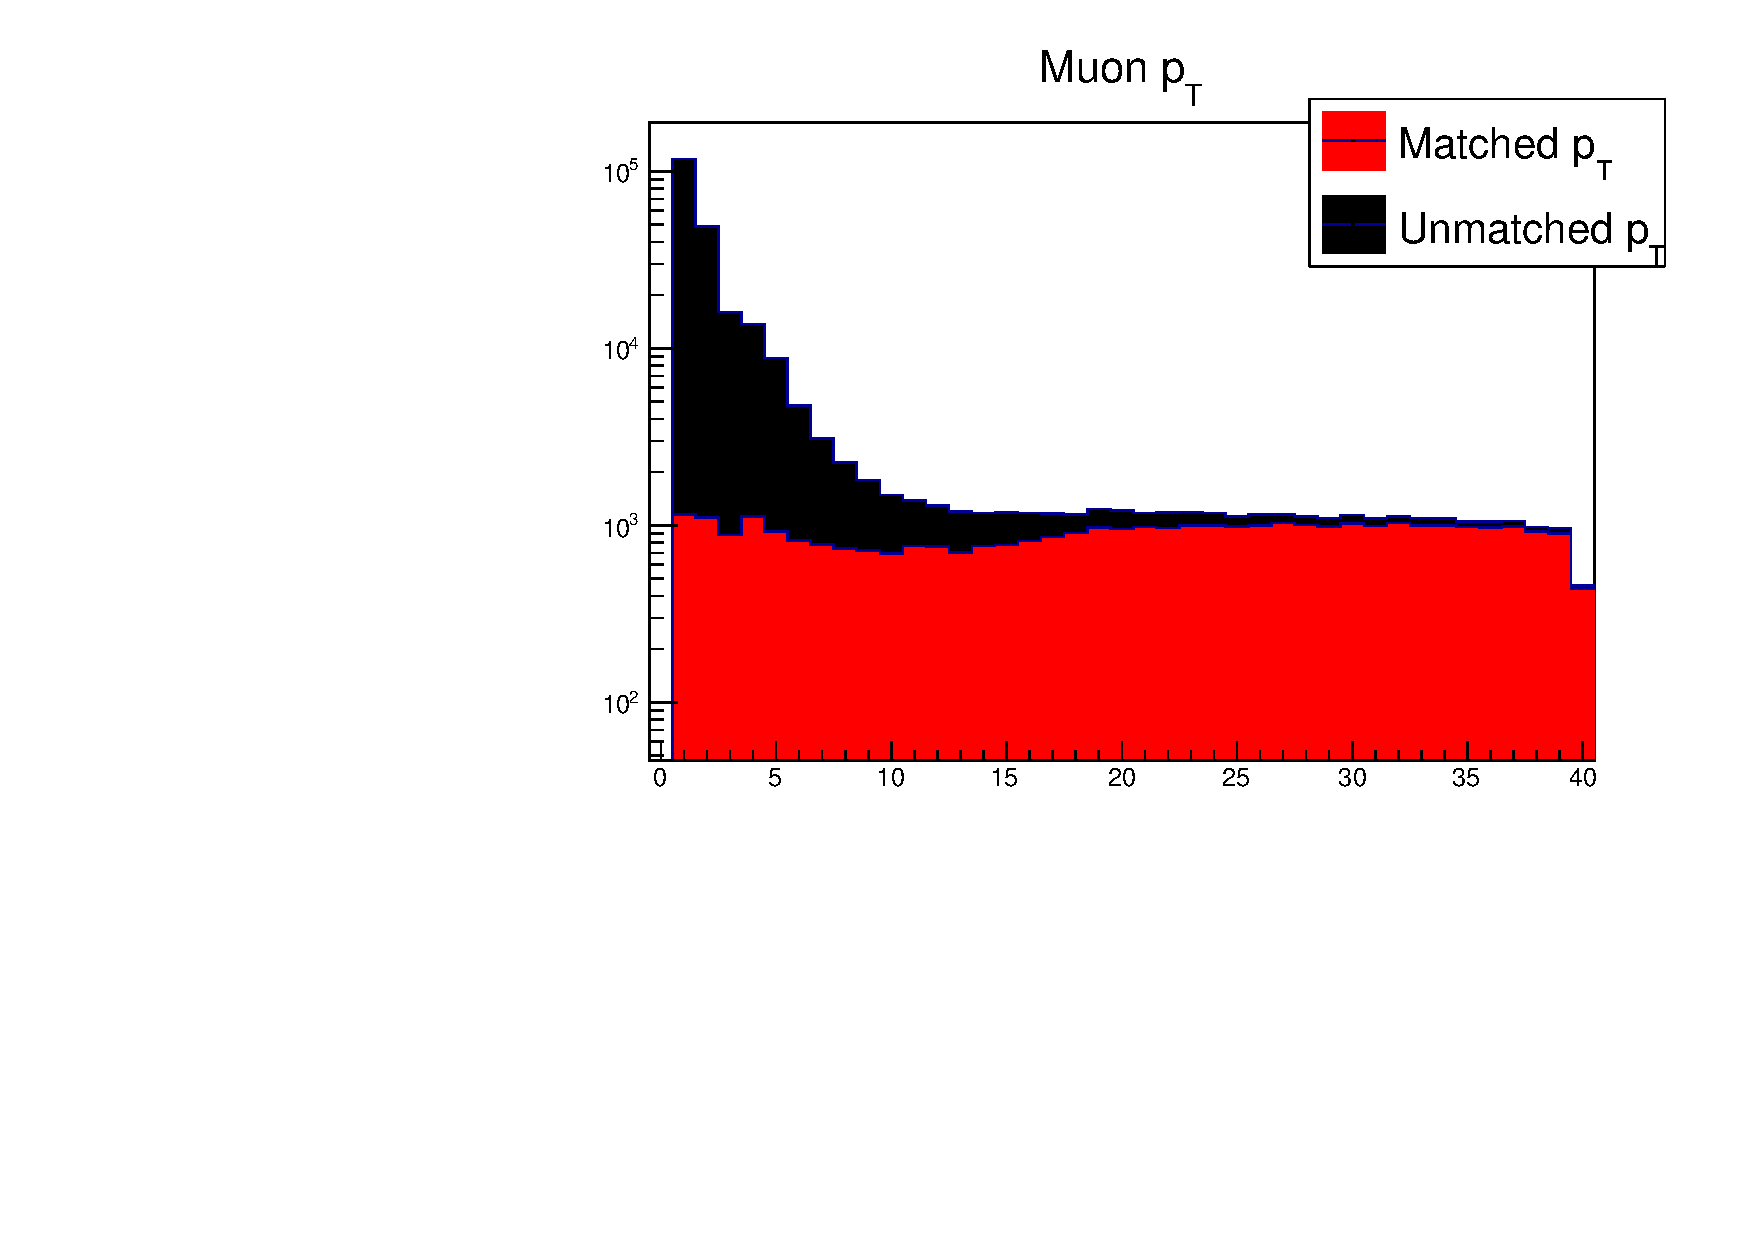
\includegraphics[scale=.3]{dy_pt.pdf}

\end{column}
\begin{column}{0.5\textwidth}
Reconstructed $p_T > 2 $ GeV
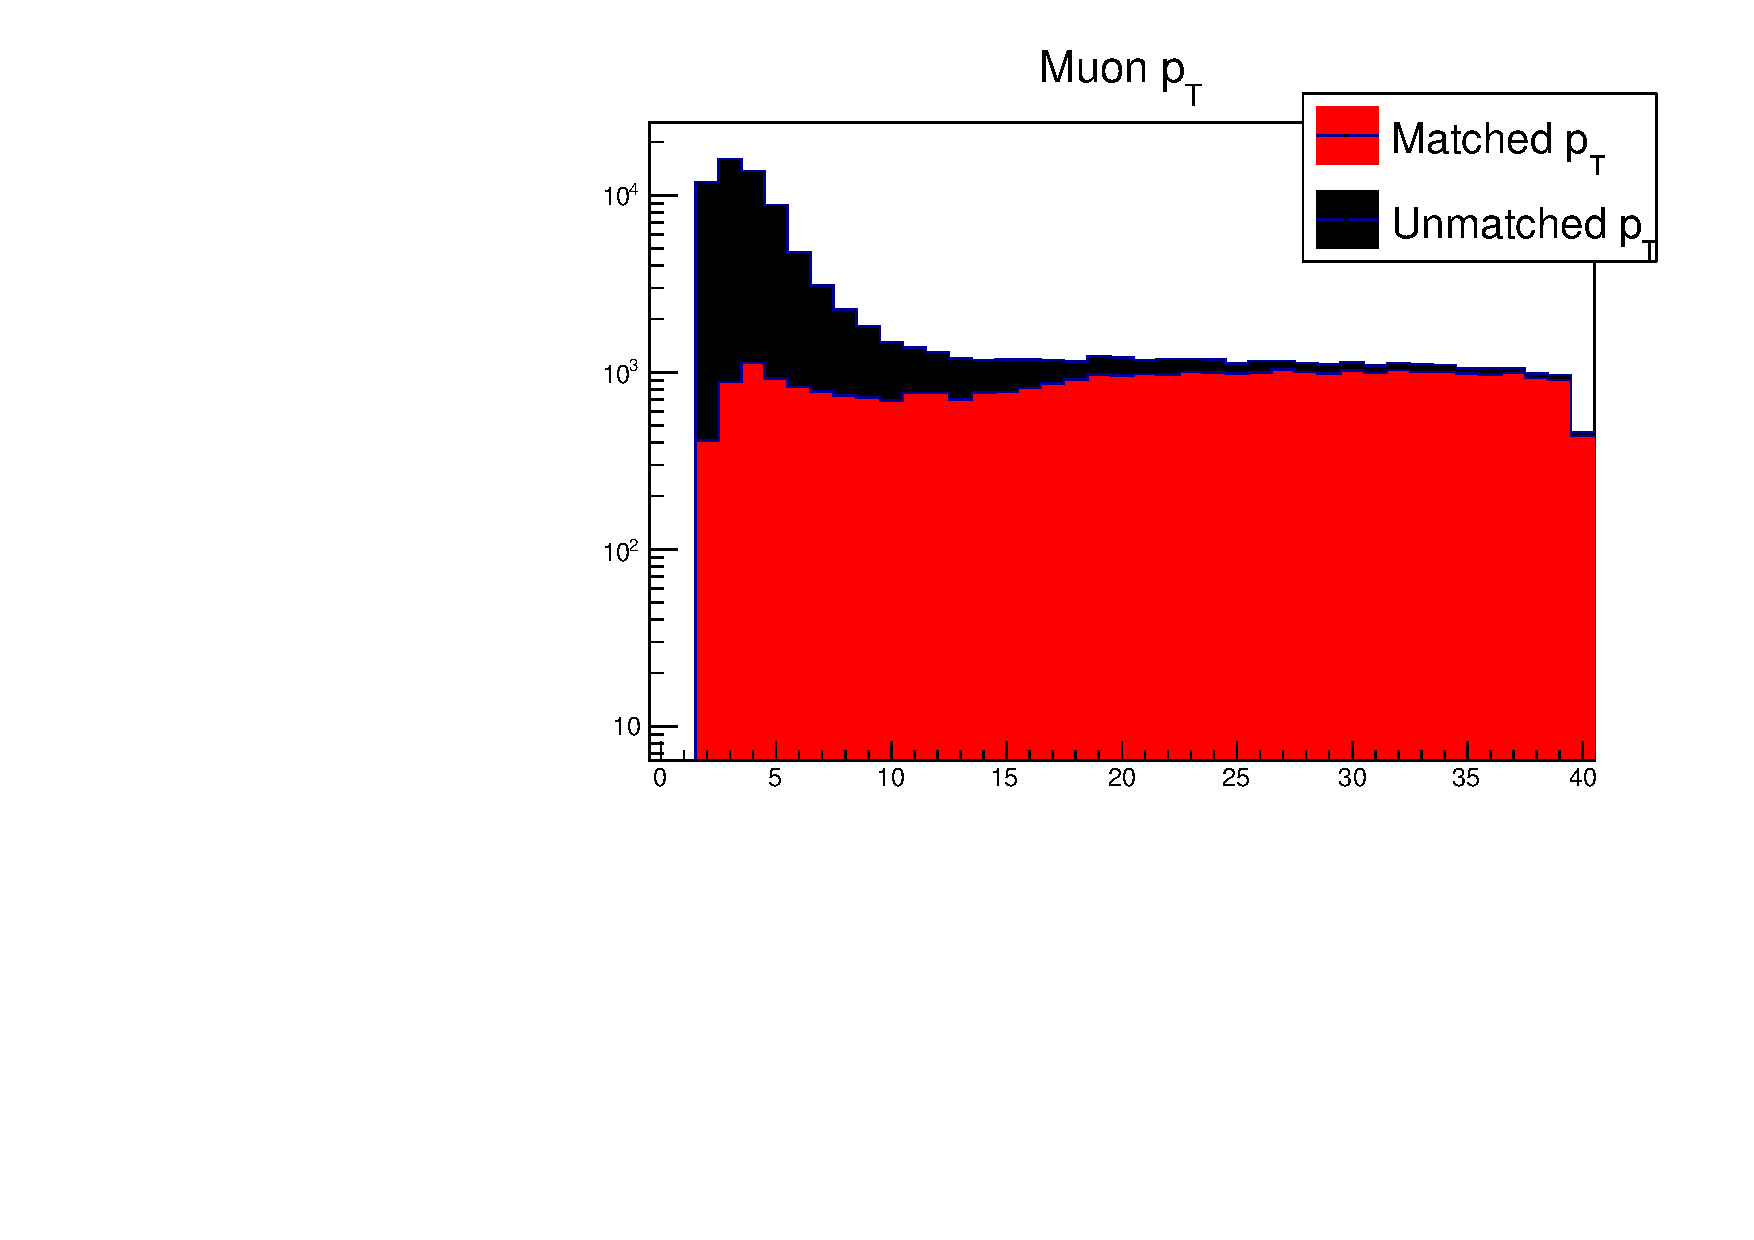
\includegraphics[scale=.3]{dy_ptcut.pdf}
\end{column}
\end{columns}

\begin{itemize}
\item many unmatchable junk muons at very low pT
\item apply a simple pt cut to clean up 
\end{itemize}
\end{frame}

\begin{frame}{ DY } 

\quad \quad \\
\begin{columns}
\begin{column}{0.5\textwidth}
No Cut
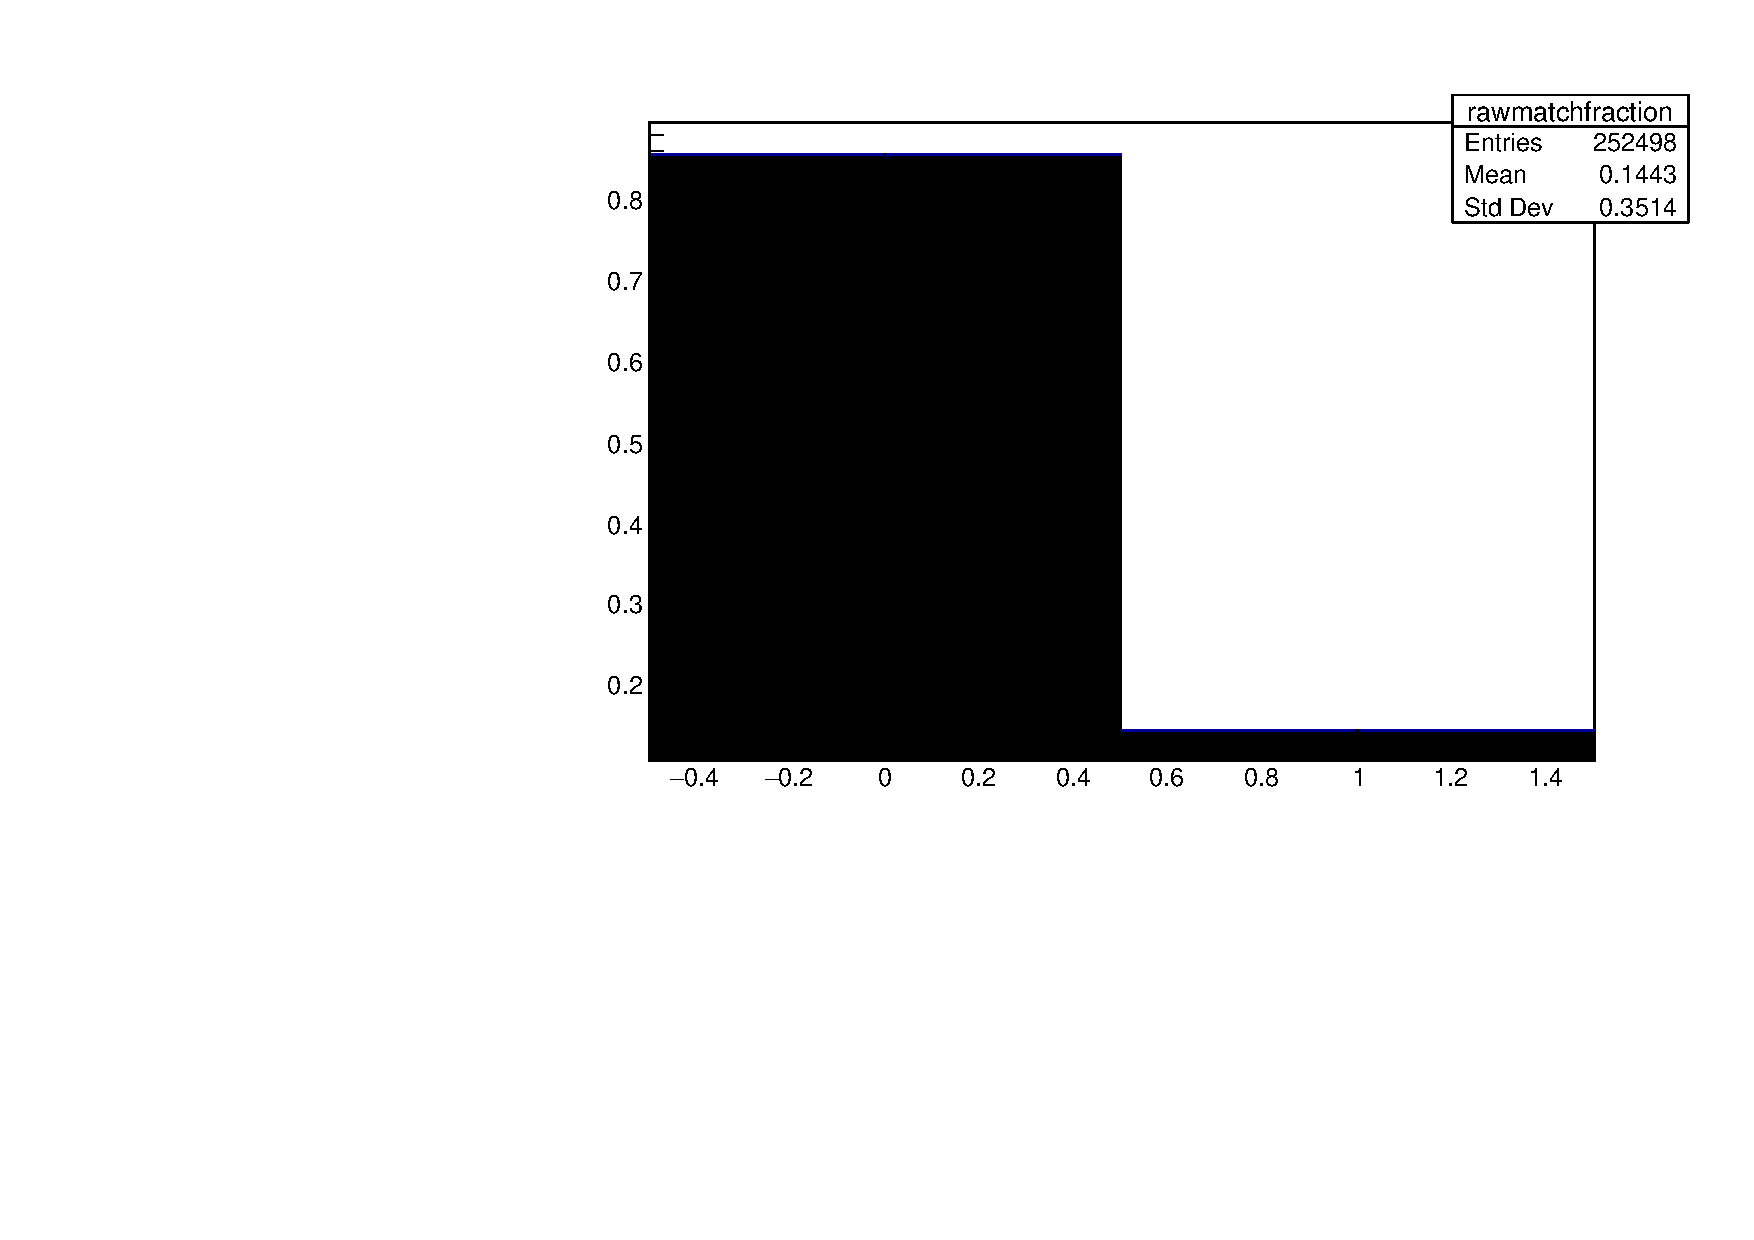
\includegraphics[scale=.3]{dy_rawmfrac.pdf}

\end{column}
\begin{column}{0.5\textwidth}
Reconstructed $p_T > 2 $ GeV
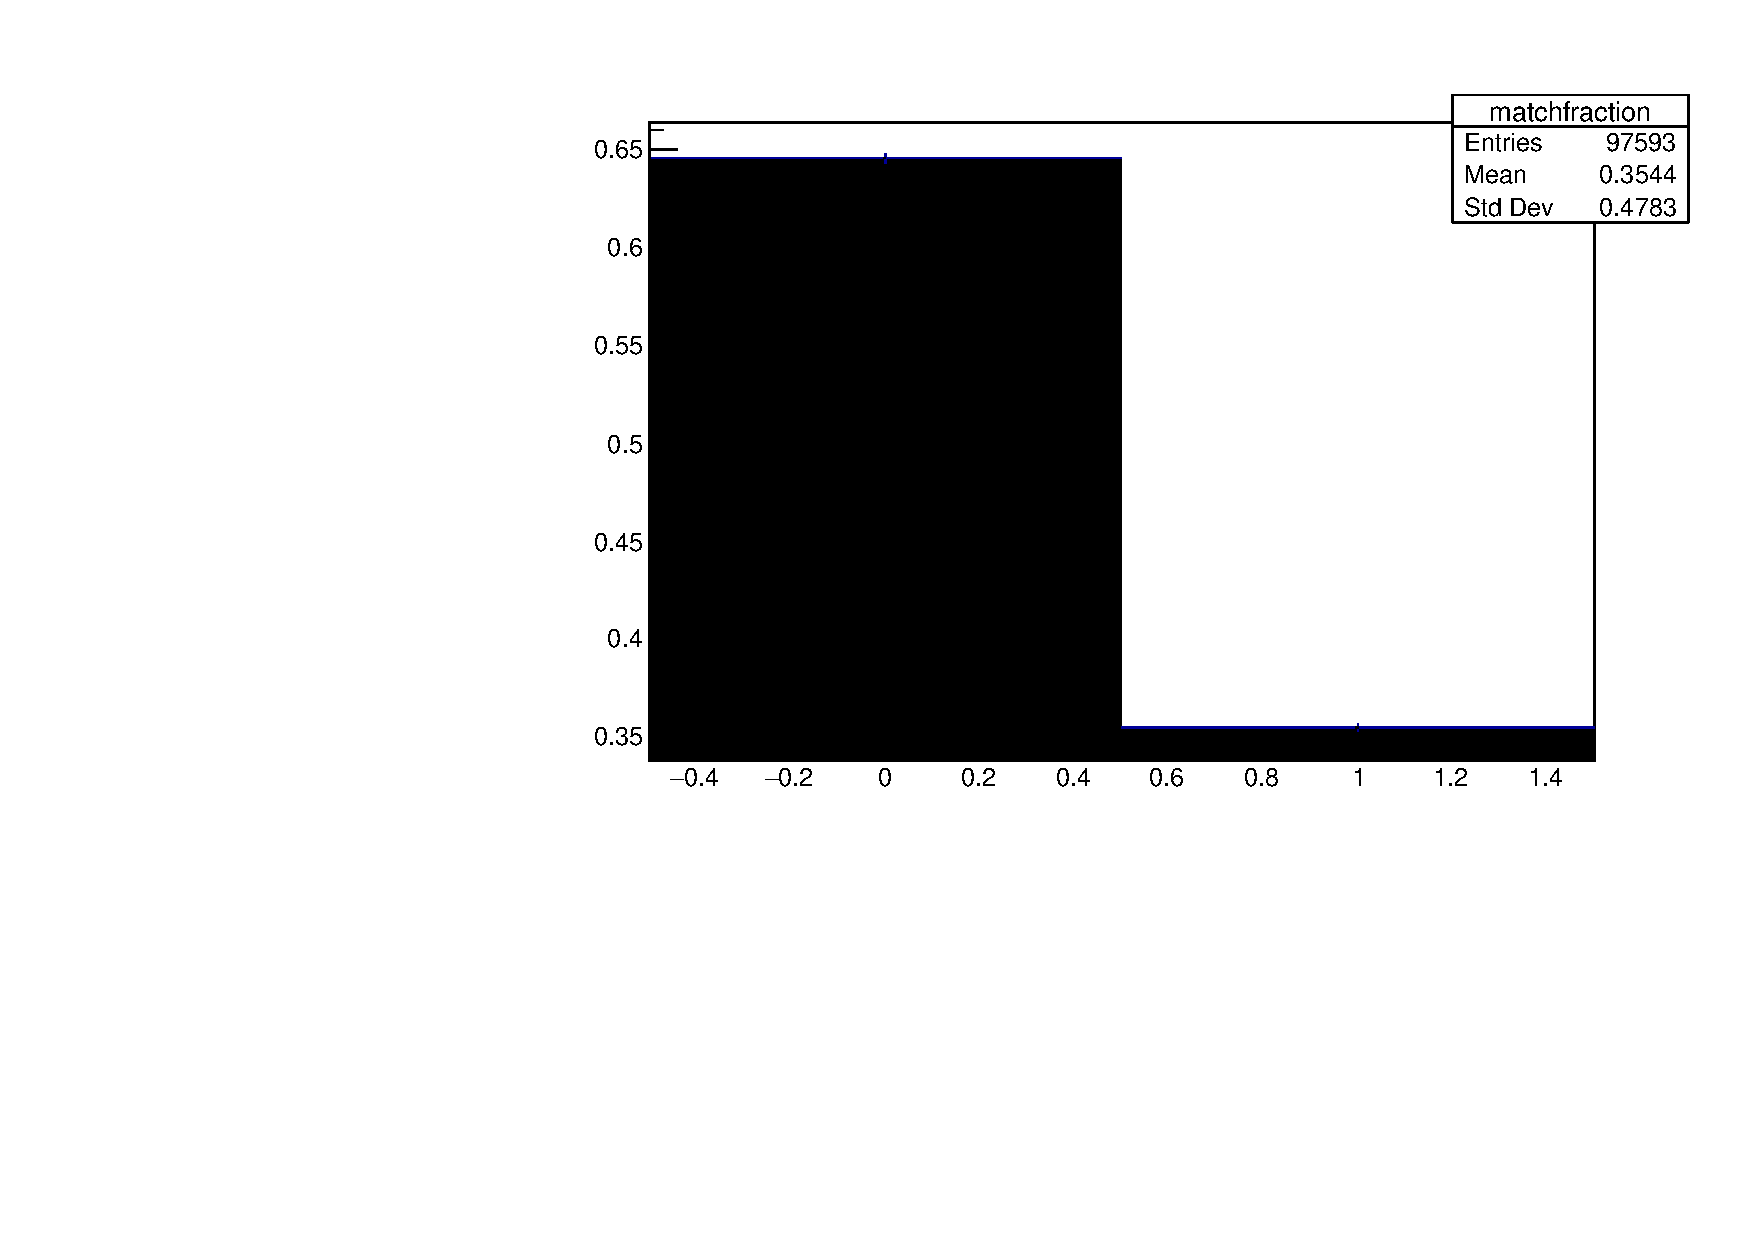
\includegraphics[scale=.3]{dy_mfrac.pdf}
\end{column}
\end{columns}


\end{frame}


\begin{frame}{ DY } 

\quad \quad \\
\begin{columns}
\begin{column}{0.5\textwidth}

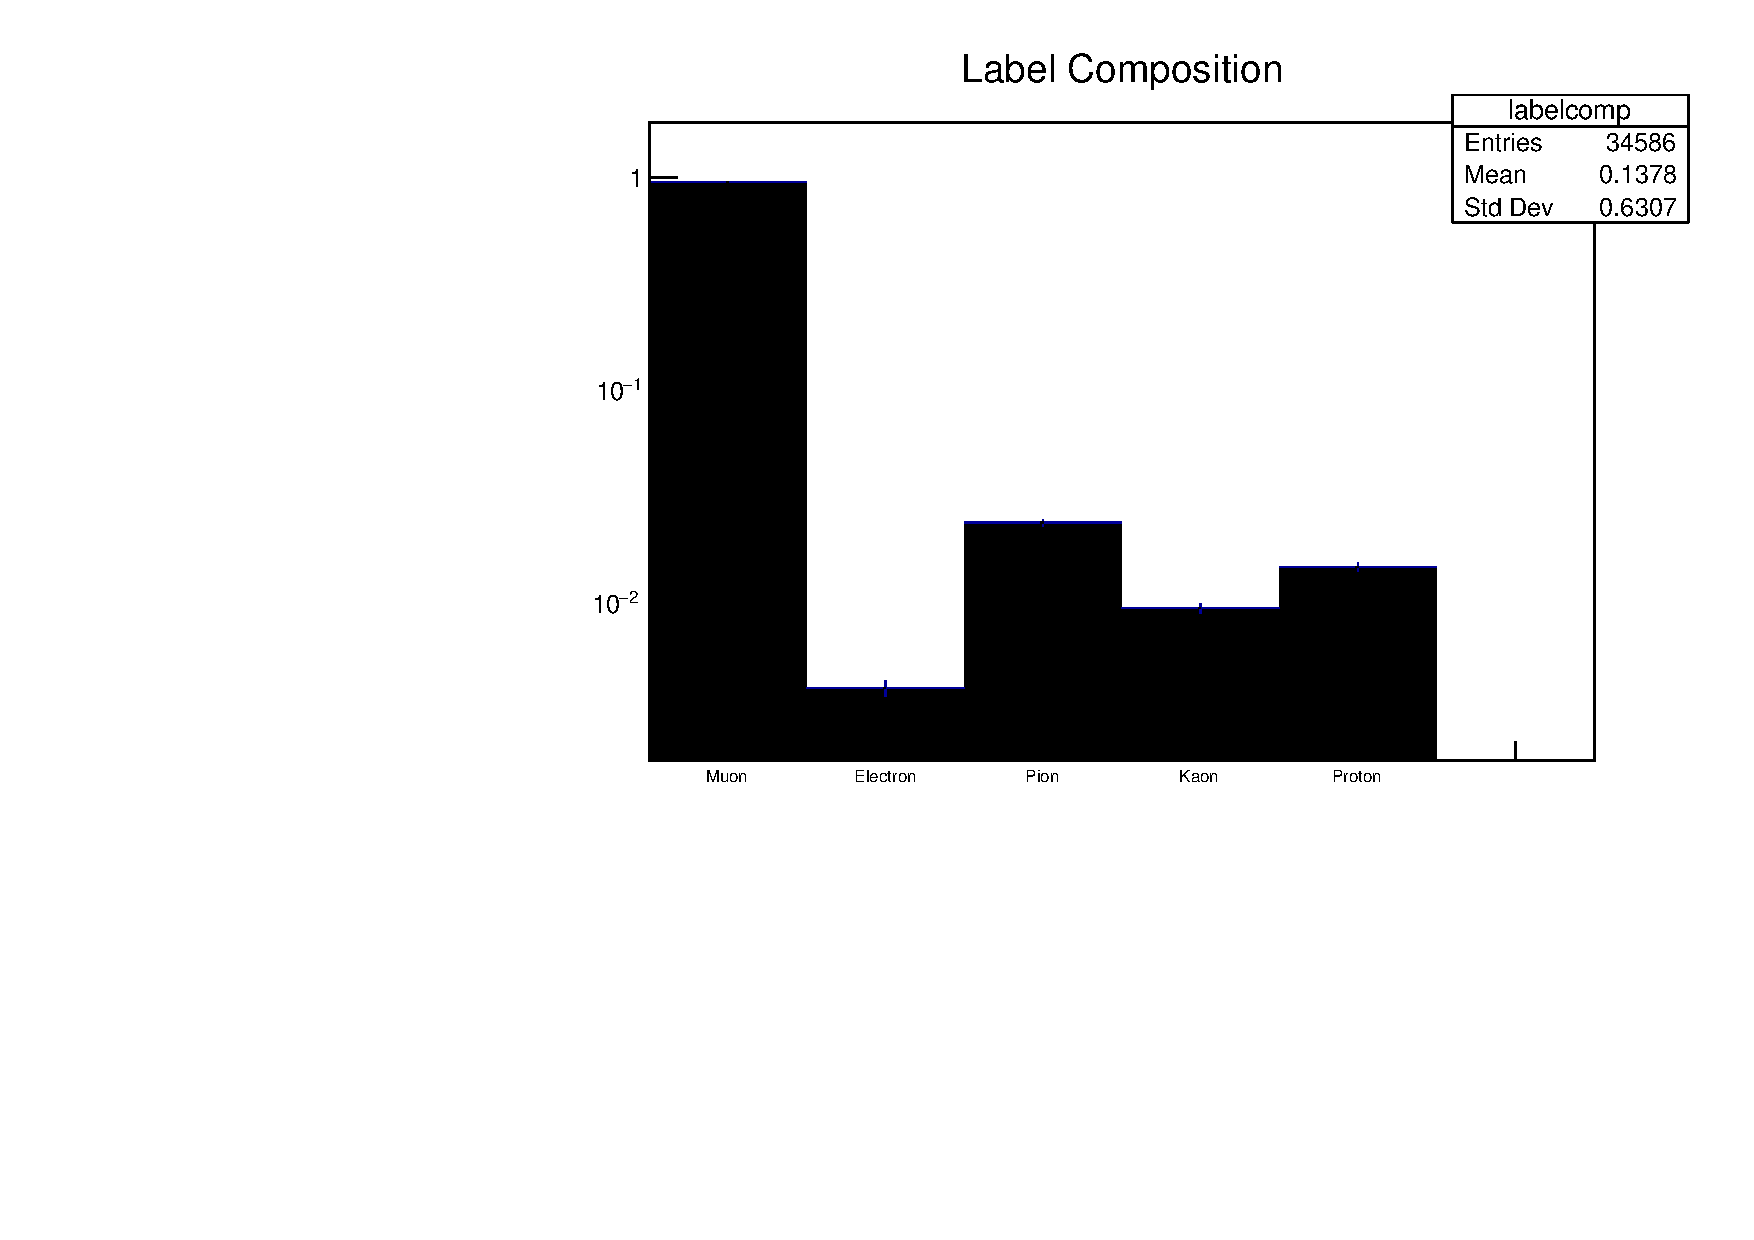
\includegraphics[scale=.3]{dy_comp.pdf}
\end{column}
\begin{column}{0.5\textwidth}

\begin{itemize}
\item From all matched particles, what is their true label
\item normalized to unity
\end{itemize}

\end{column}
\end{columns}

\end{frame}


\begin{frame}{ DY } 

\quad \quad \\
\begin{columns}
\begin{column}{0.5\textwidth}

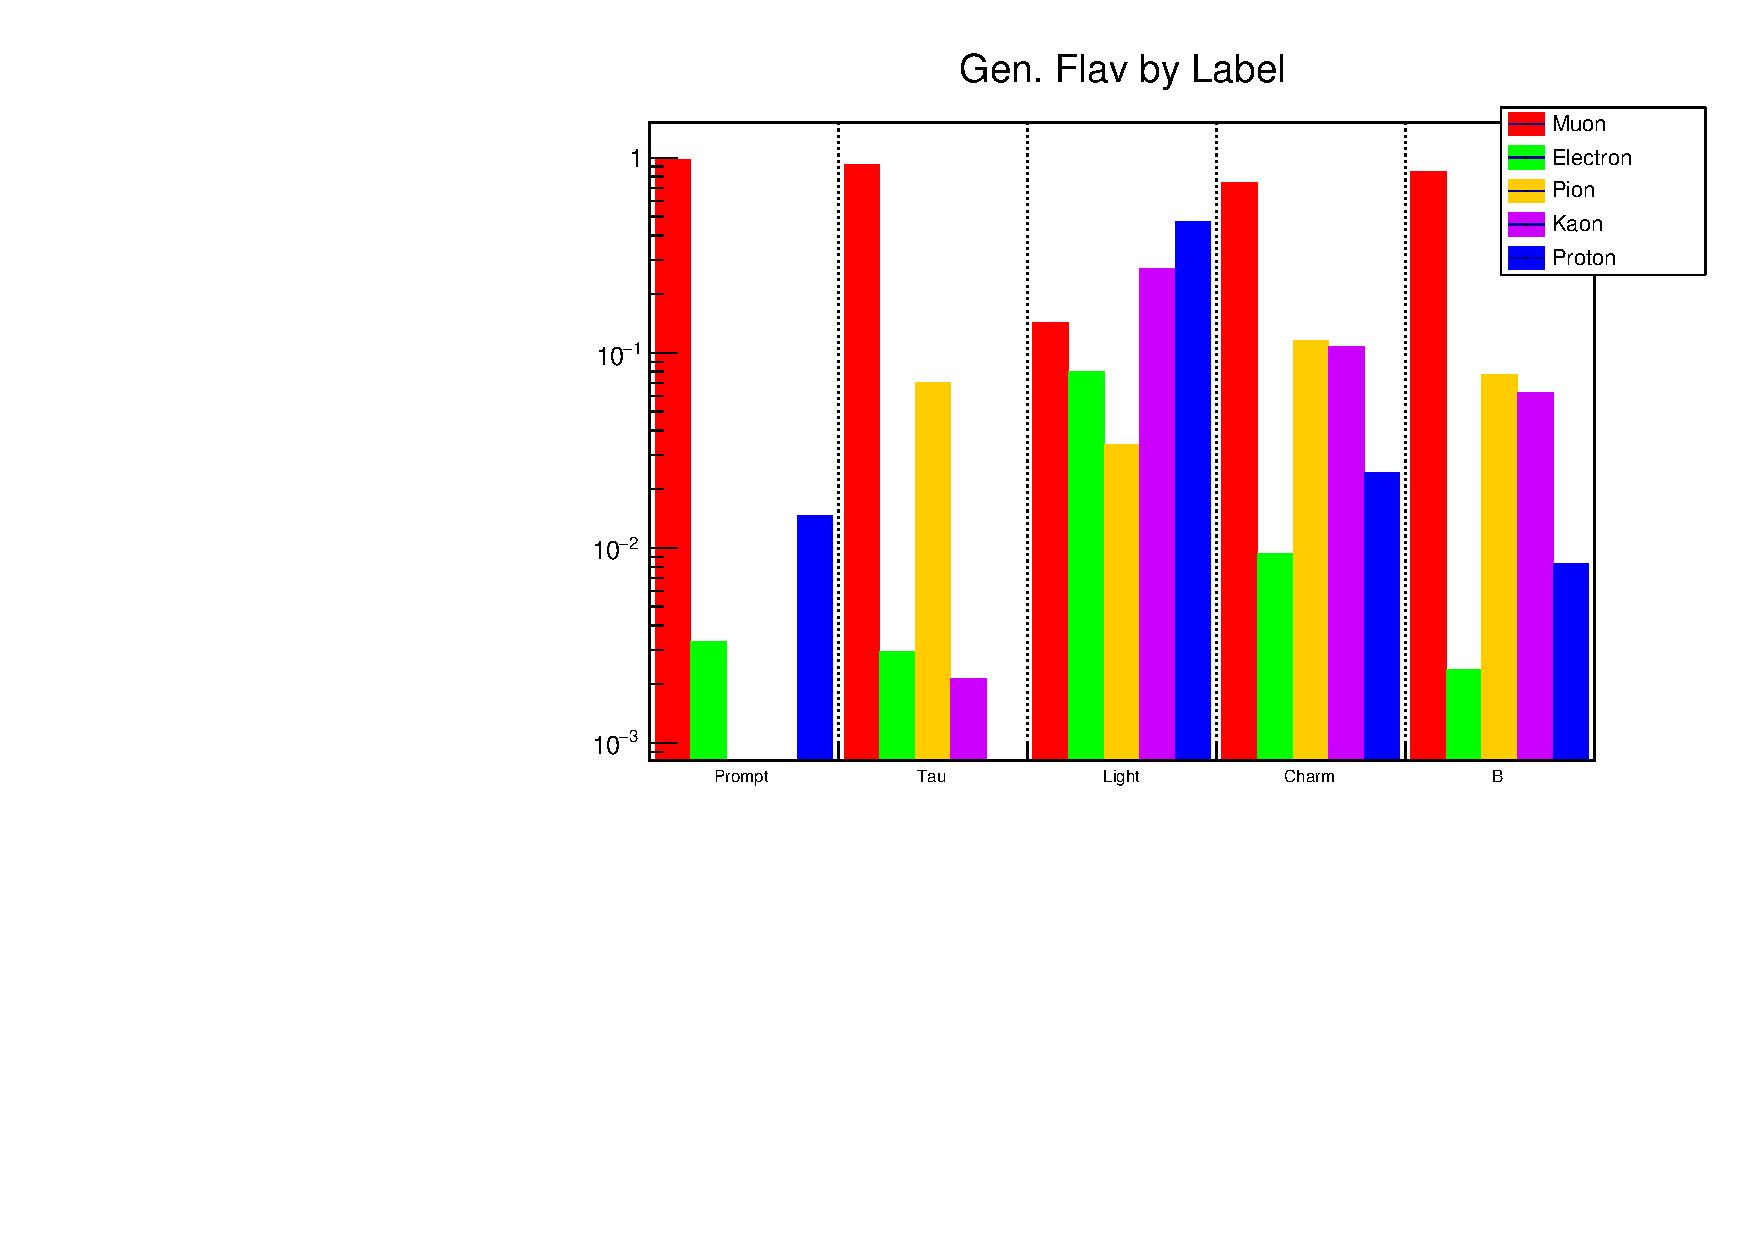
\includegraphics[scale=.3]{dy_flav.pdf}

\end{column}
\begin{column}{0.5\textwidth}
\begin{itemize}
\item Of matched particles what is their origin?
\item each flavor bin normalized to unity, by bin
\item e.g. $\%$ prompt muons = $\frac{\text{N prompt muons}}{ \text{N all labels which are prompt}}$
\end{itemize}
%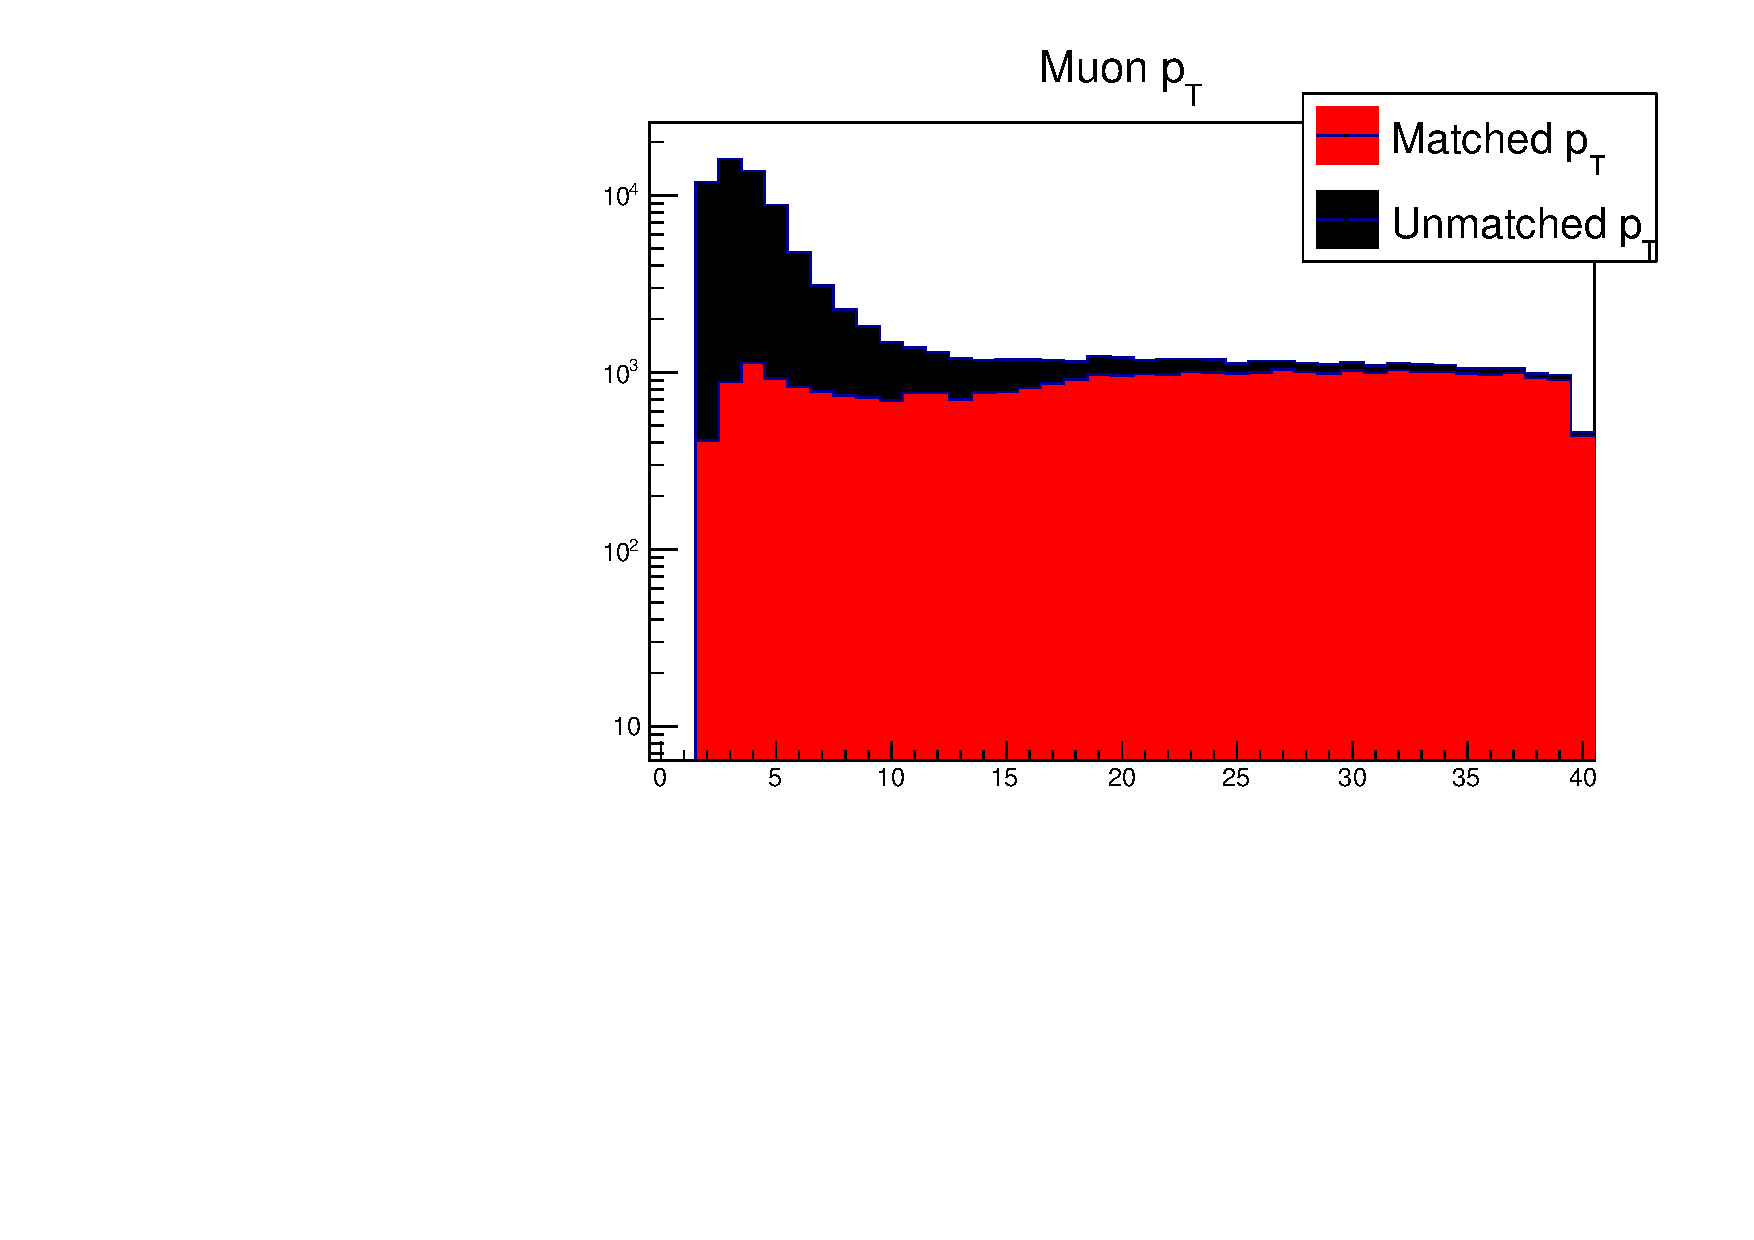
\includegraphics[scale=.3]{dy_ptcut.pdf}
\end{column}
\end{columns}
\end{frame}

\begin{frame}{ DY } 

\quad \quad \\
\begin{columns}
\begin{column}{0.5\textwidth}

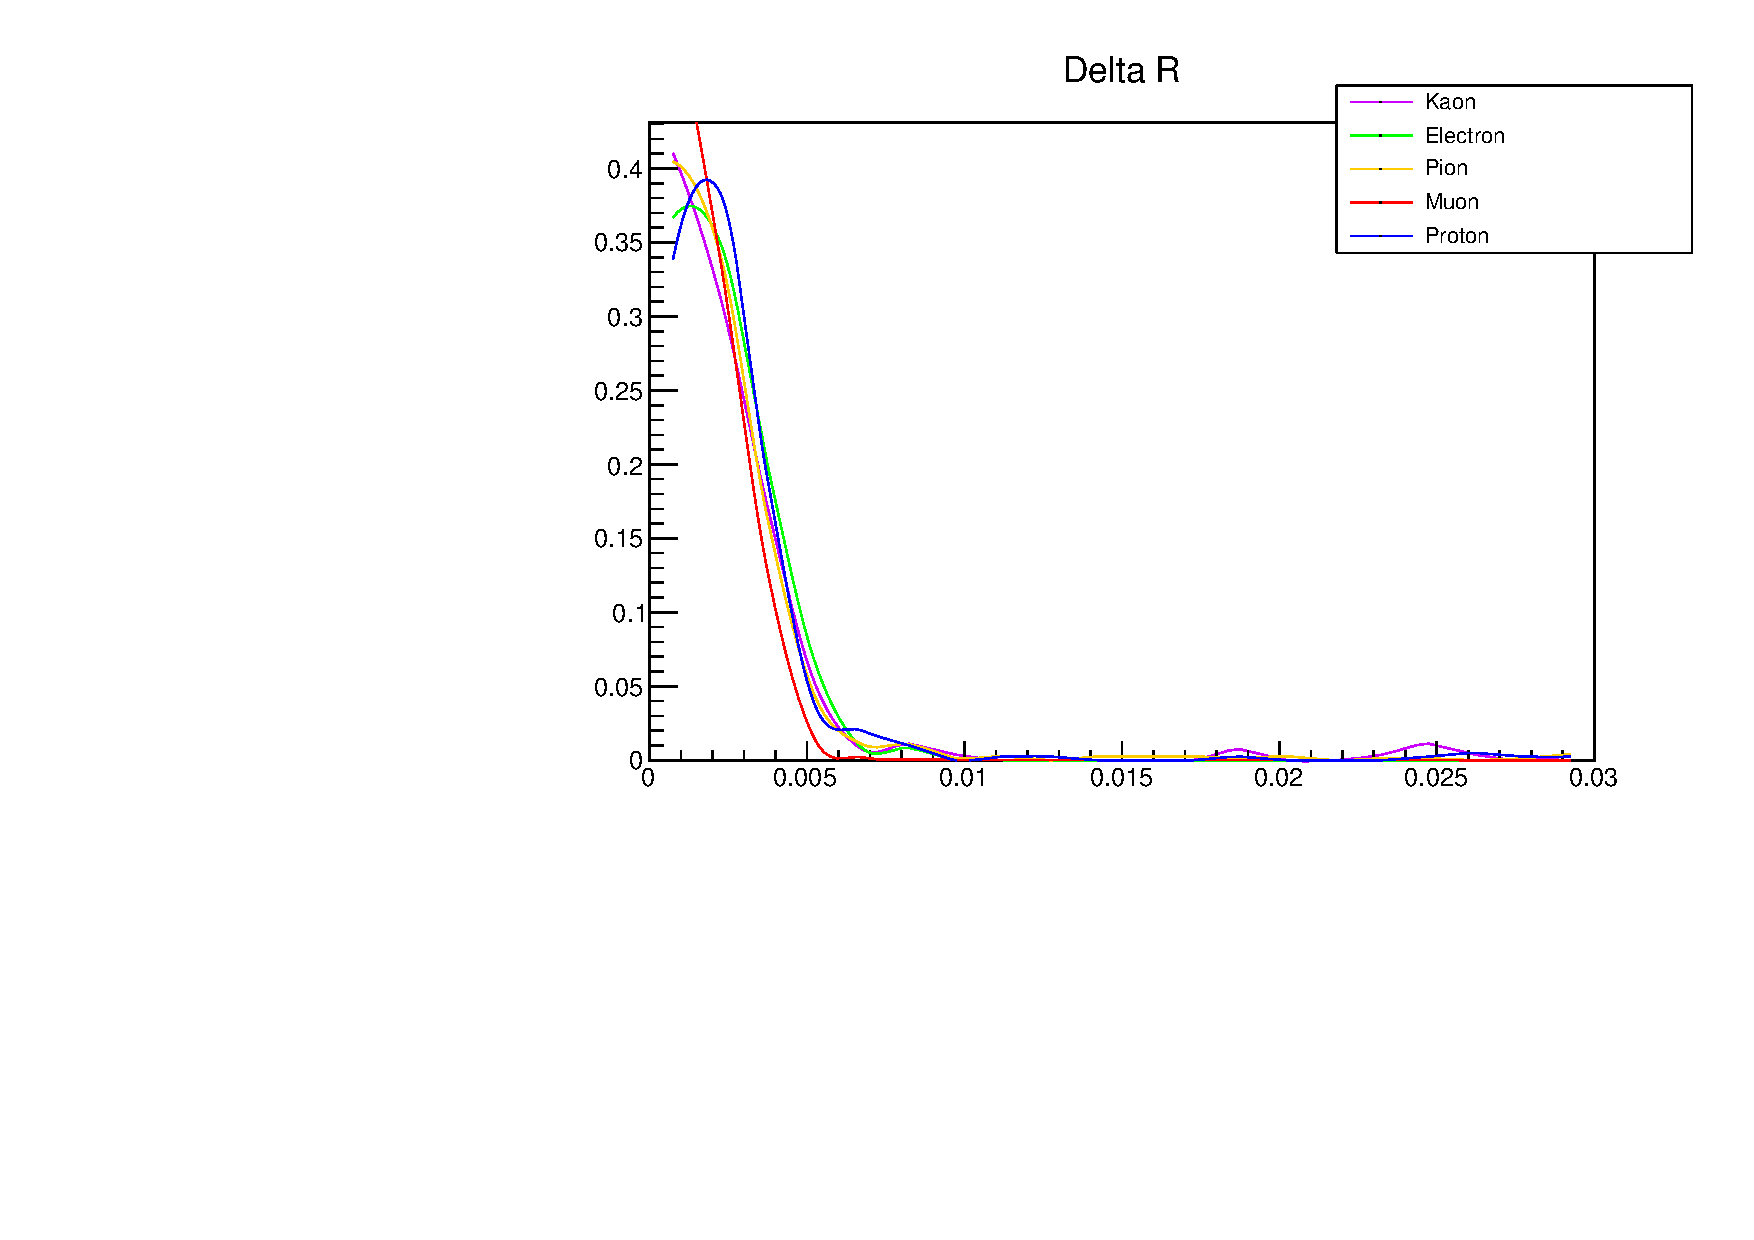
\includegraphics[scale=.3]{dy_dr.pdf}

\end{column}
\begin{column}{0.5\textwidth}

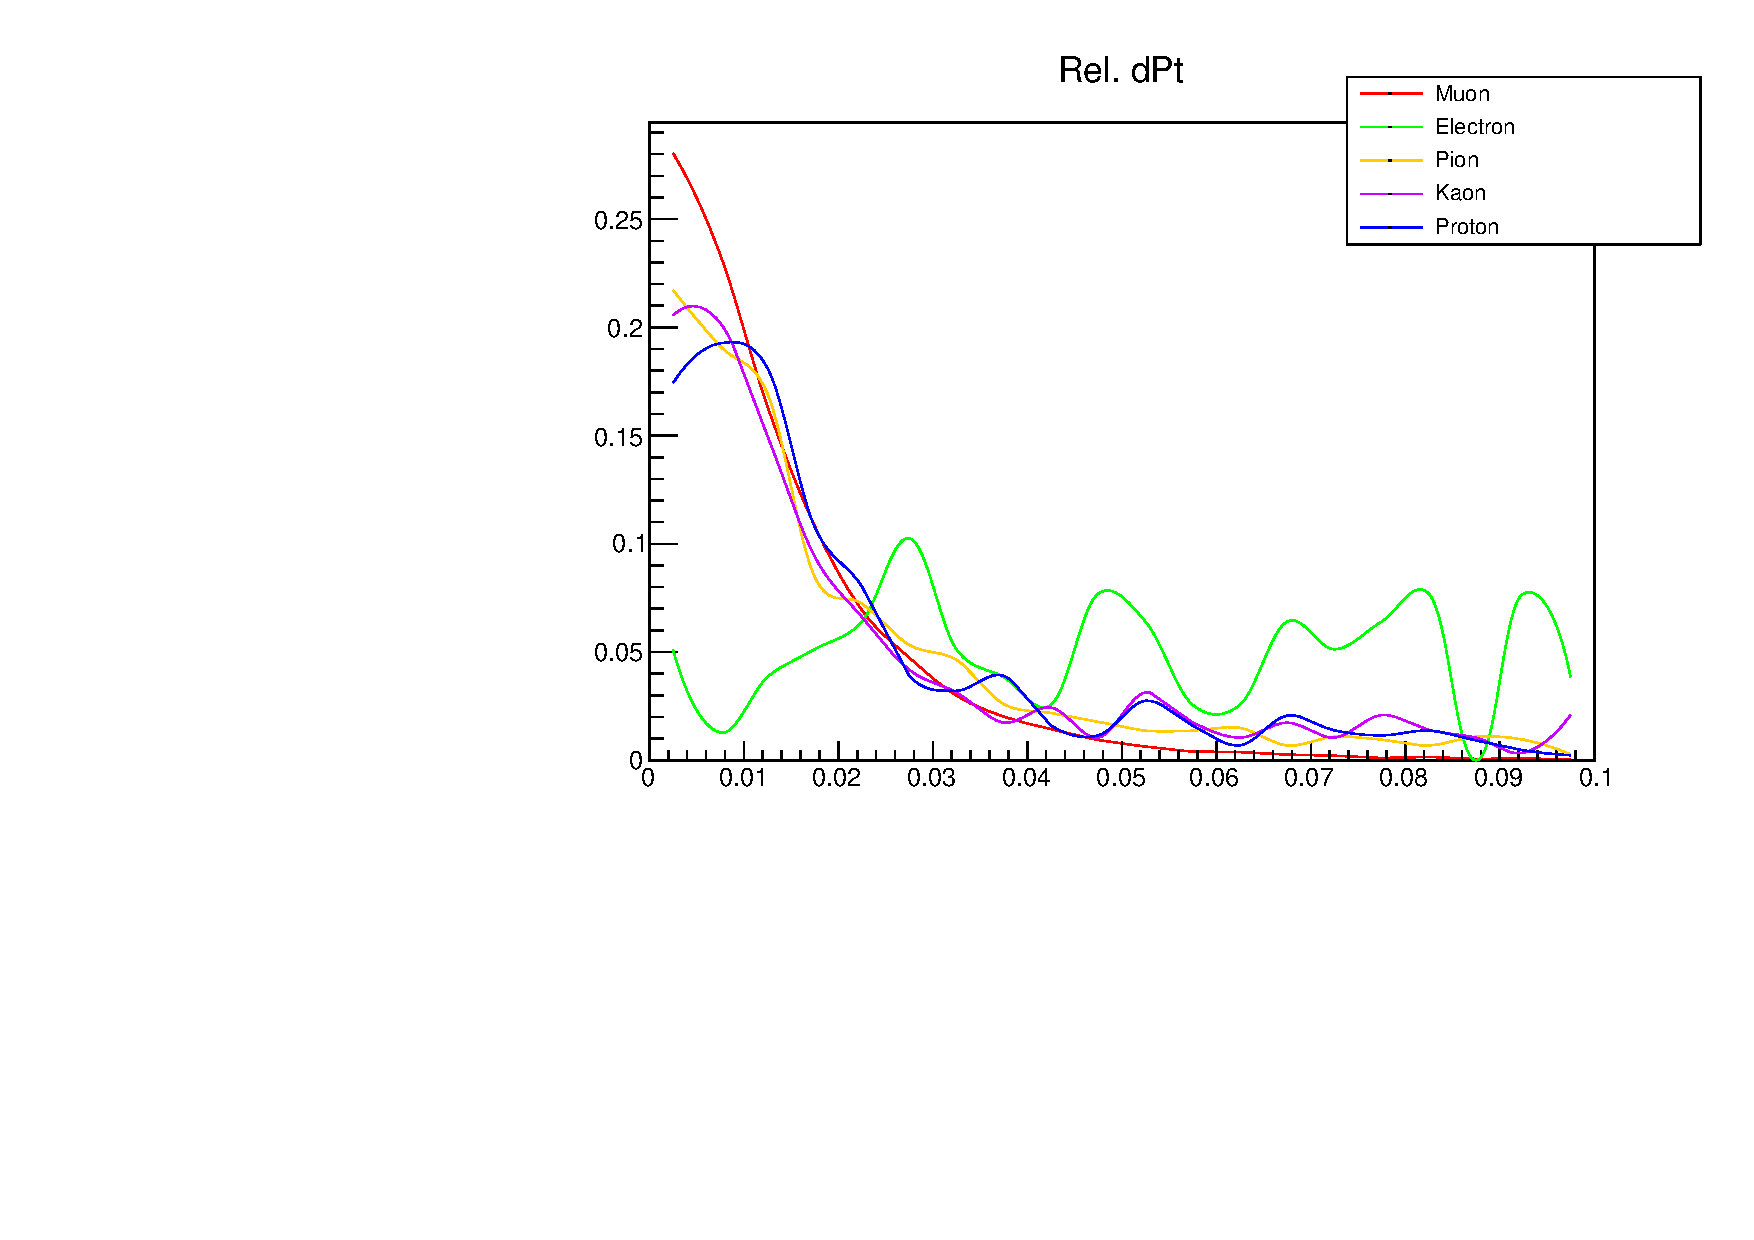
\includegraphics[scale=.3]{dy_dptrel.pdf}
\end{column}
\end{columns}
\end{frame}

\begin{frame}{ TT } 

\quad \quad \\
\begin{columns}
\begin{column}{0.5\textwidth}
No Cut
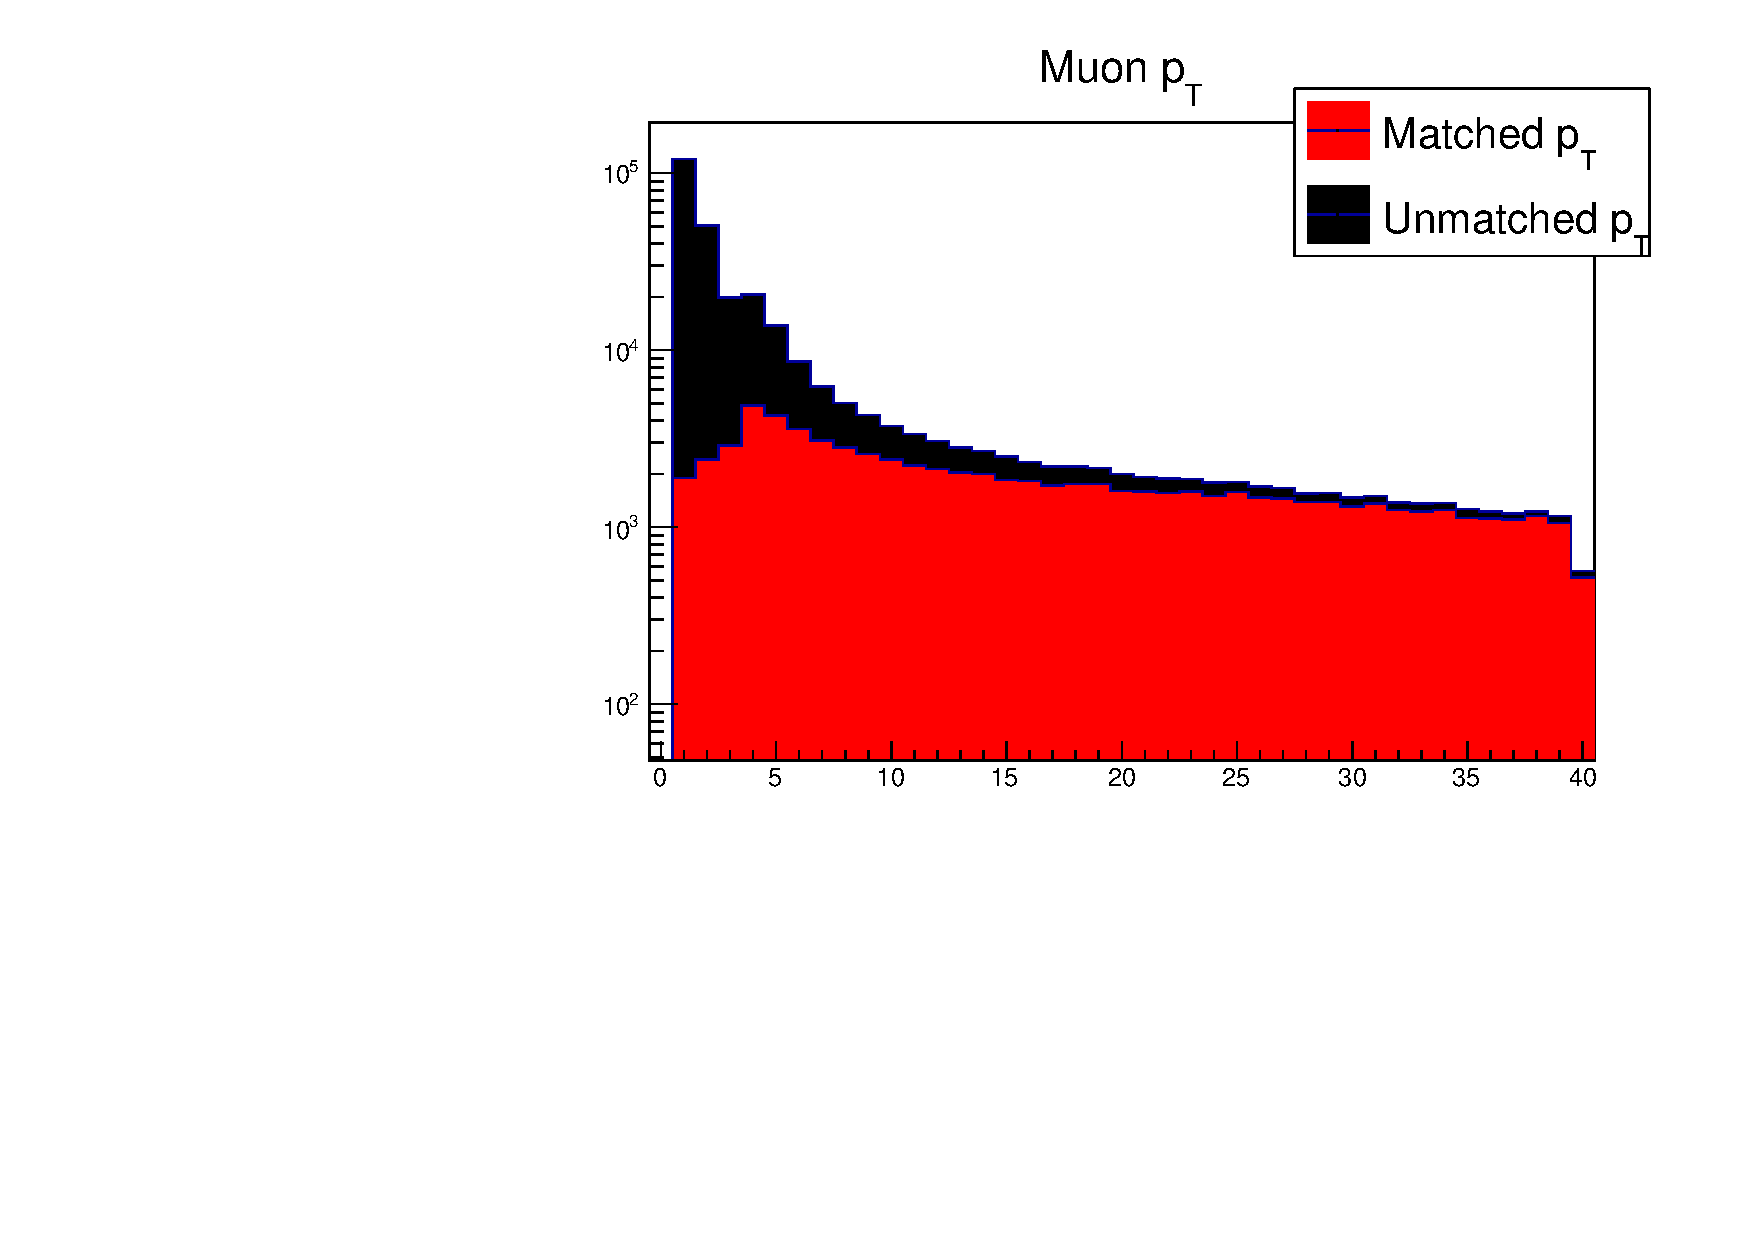
\includegraphics[scale=.3]{tt_pt.pdf}

\end{column}
\begin{column}{0.5\textwidth}
Reconstructed $p_T > 2 $ GeV
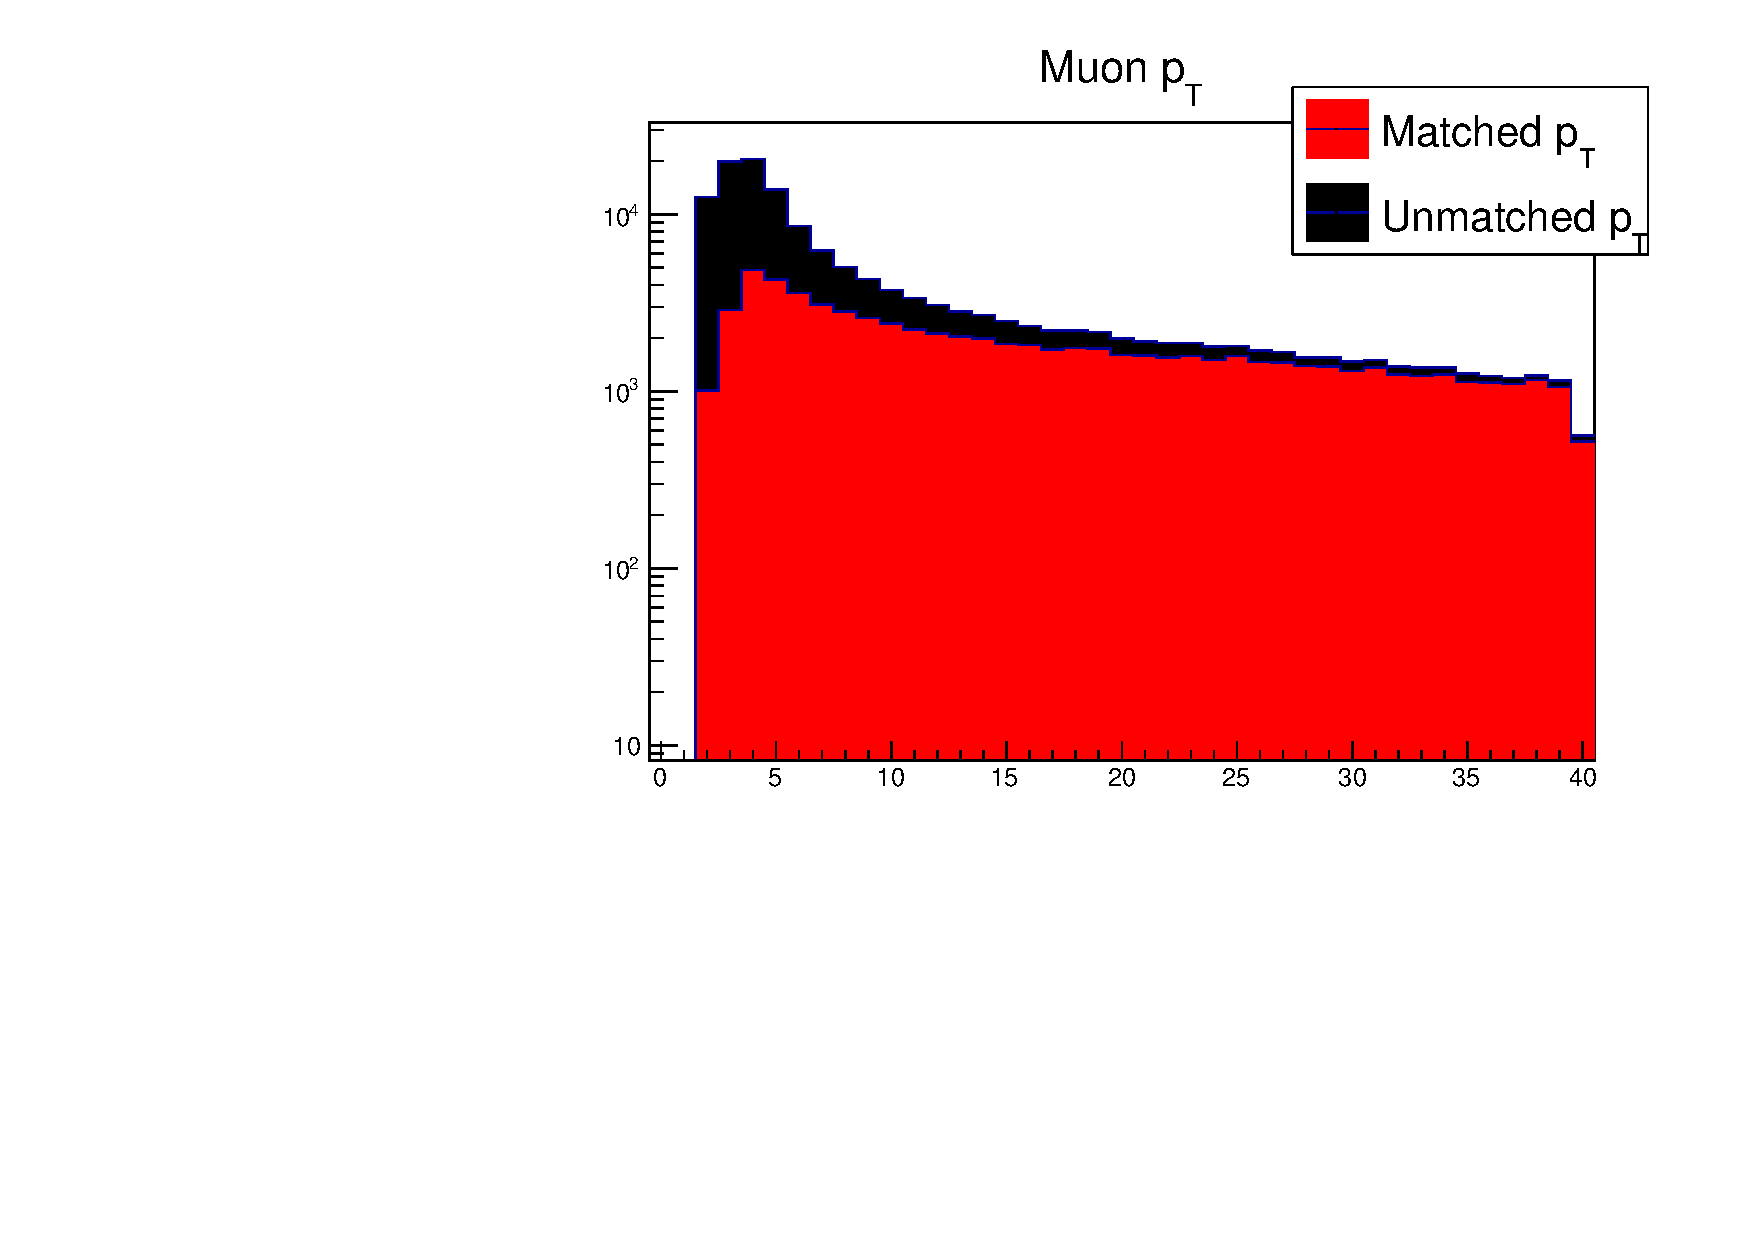
\includegraphics[scale=.3]{tt_ptcut.pdf}
\end{column}
\end{columns}
\end{frame}

\begin{frame}{ TT } 

\quad \quad \\
\begin{columns}
\begin{column}{0.5\textwidth}
No Cut
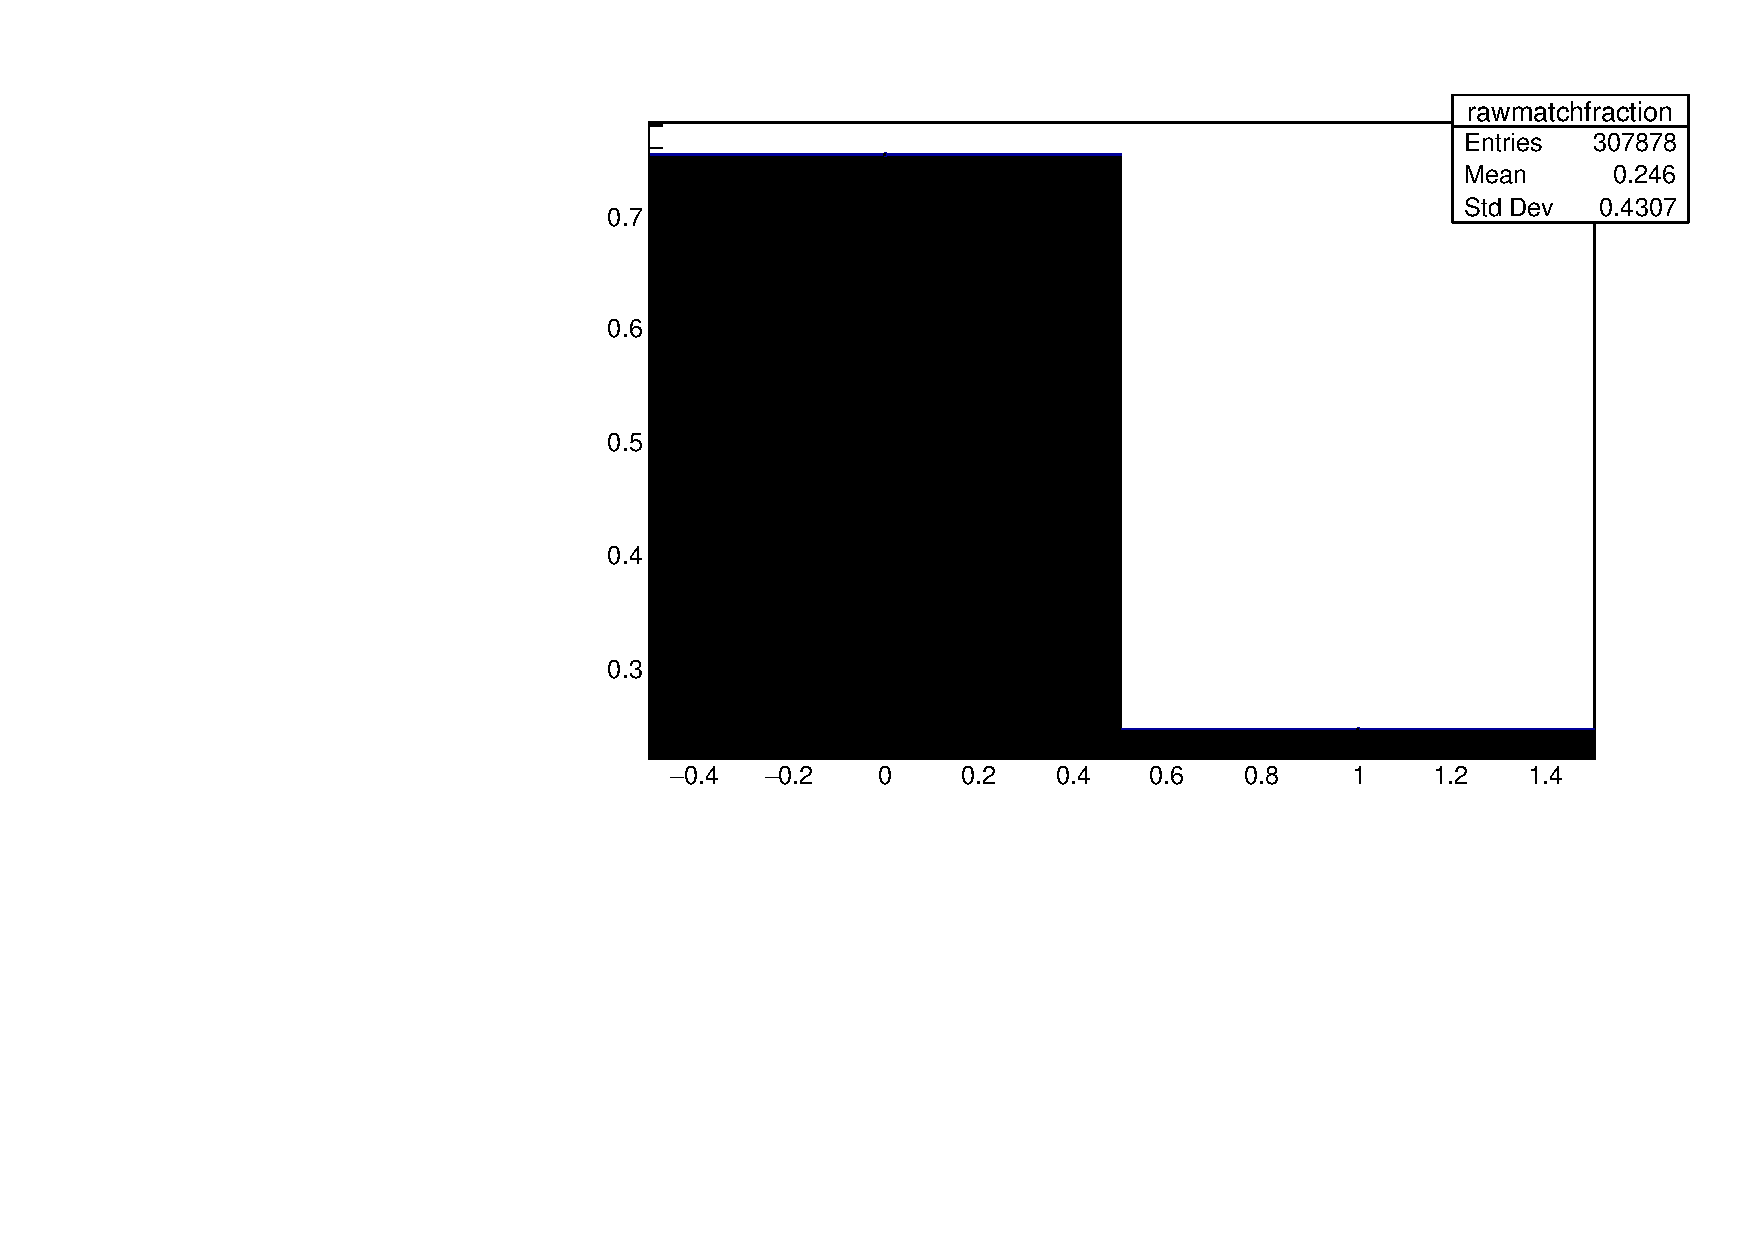
\includegraphics[scale=.3]{tt_rawmfrac.pdf}

\end{column}
\begin{column}{0.5\textwidth}
Reconstructed $p_T > 2 $ GeV
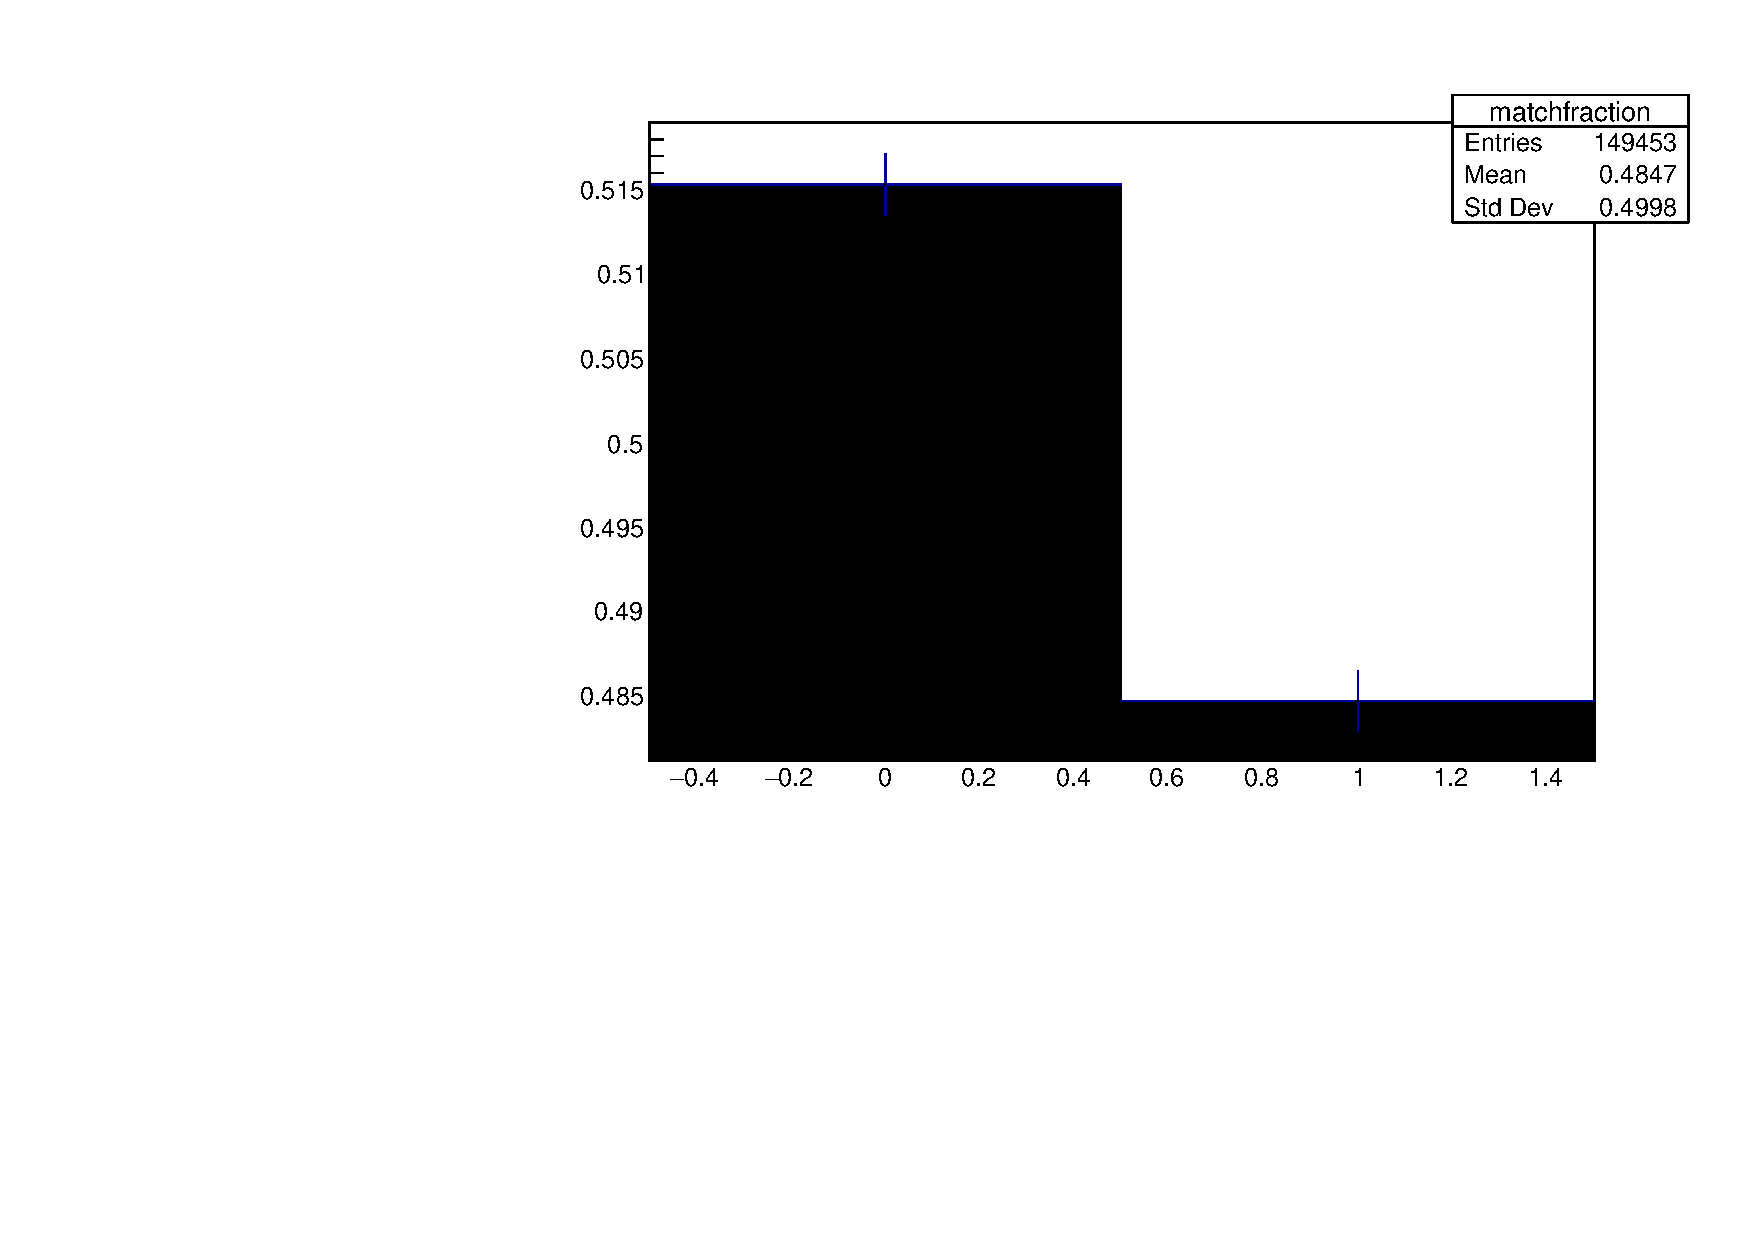
\includegraphics[scale=.3]{tt_mfrac.pdf}
\end{column}
\end{columns}


\end{frame}

\begin{frame}{ TT } 

\quad \quad \\
\begin{columns}
\begin{column}{0.5\textwidth}

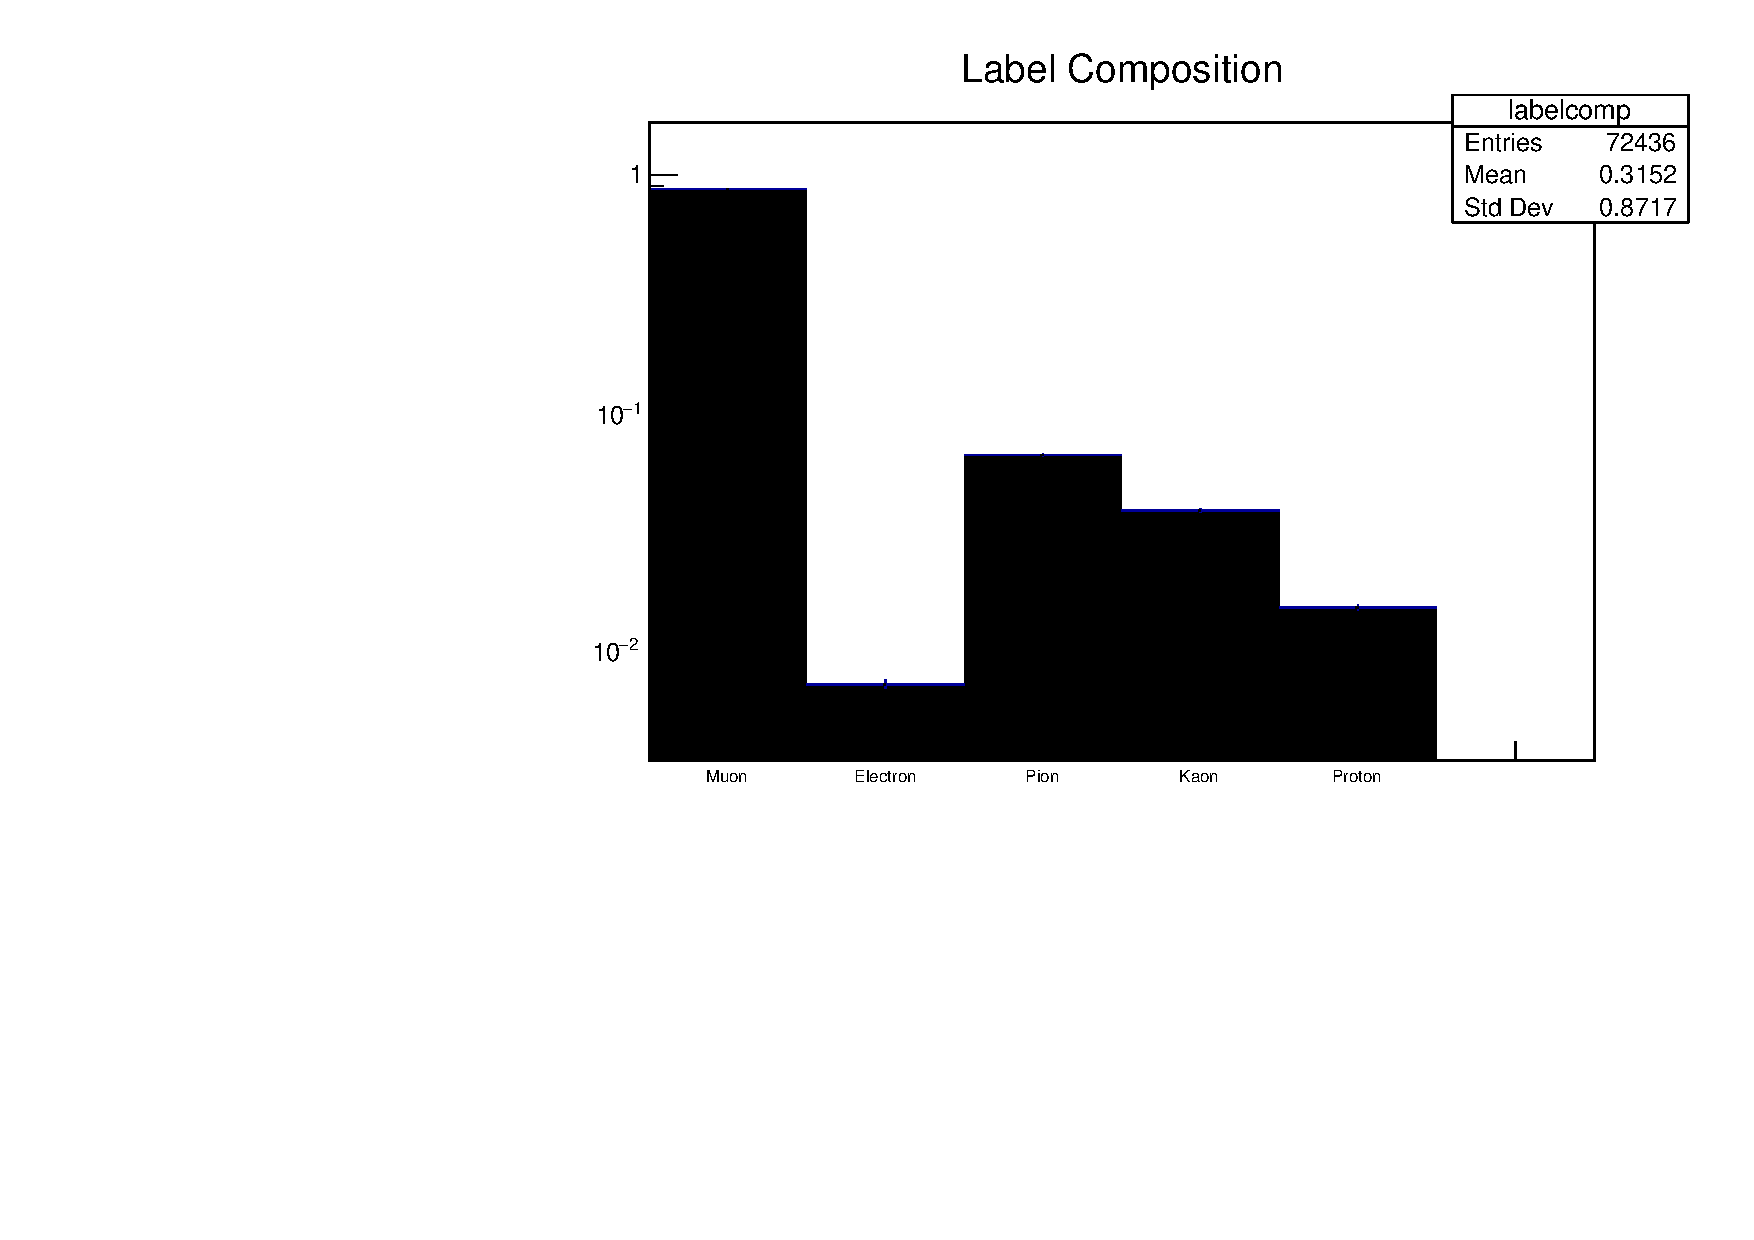
\includegraphics[scale=.3]{tt_comp.pdf}

\end{column}
\begin{column}{0.5\textwidth}

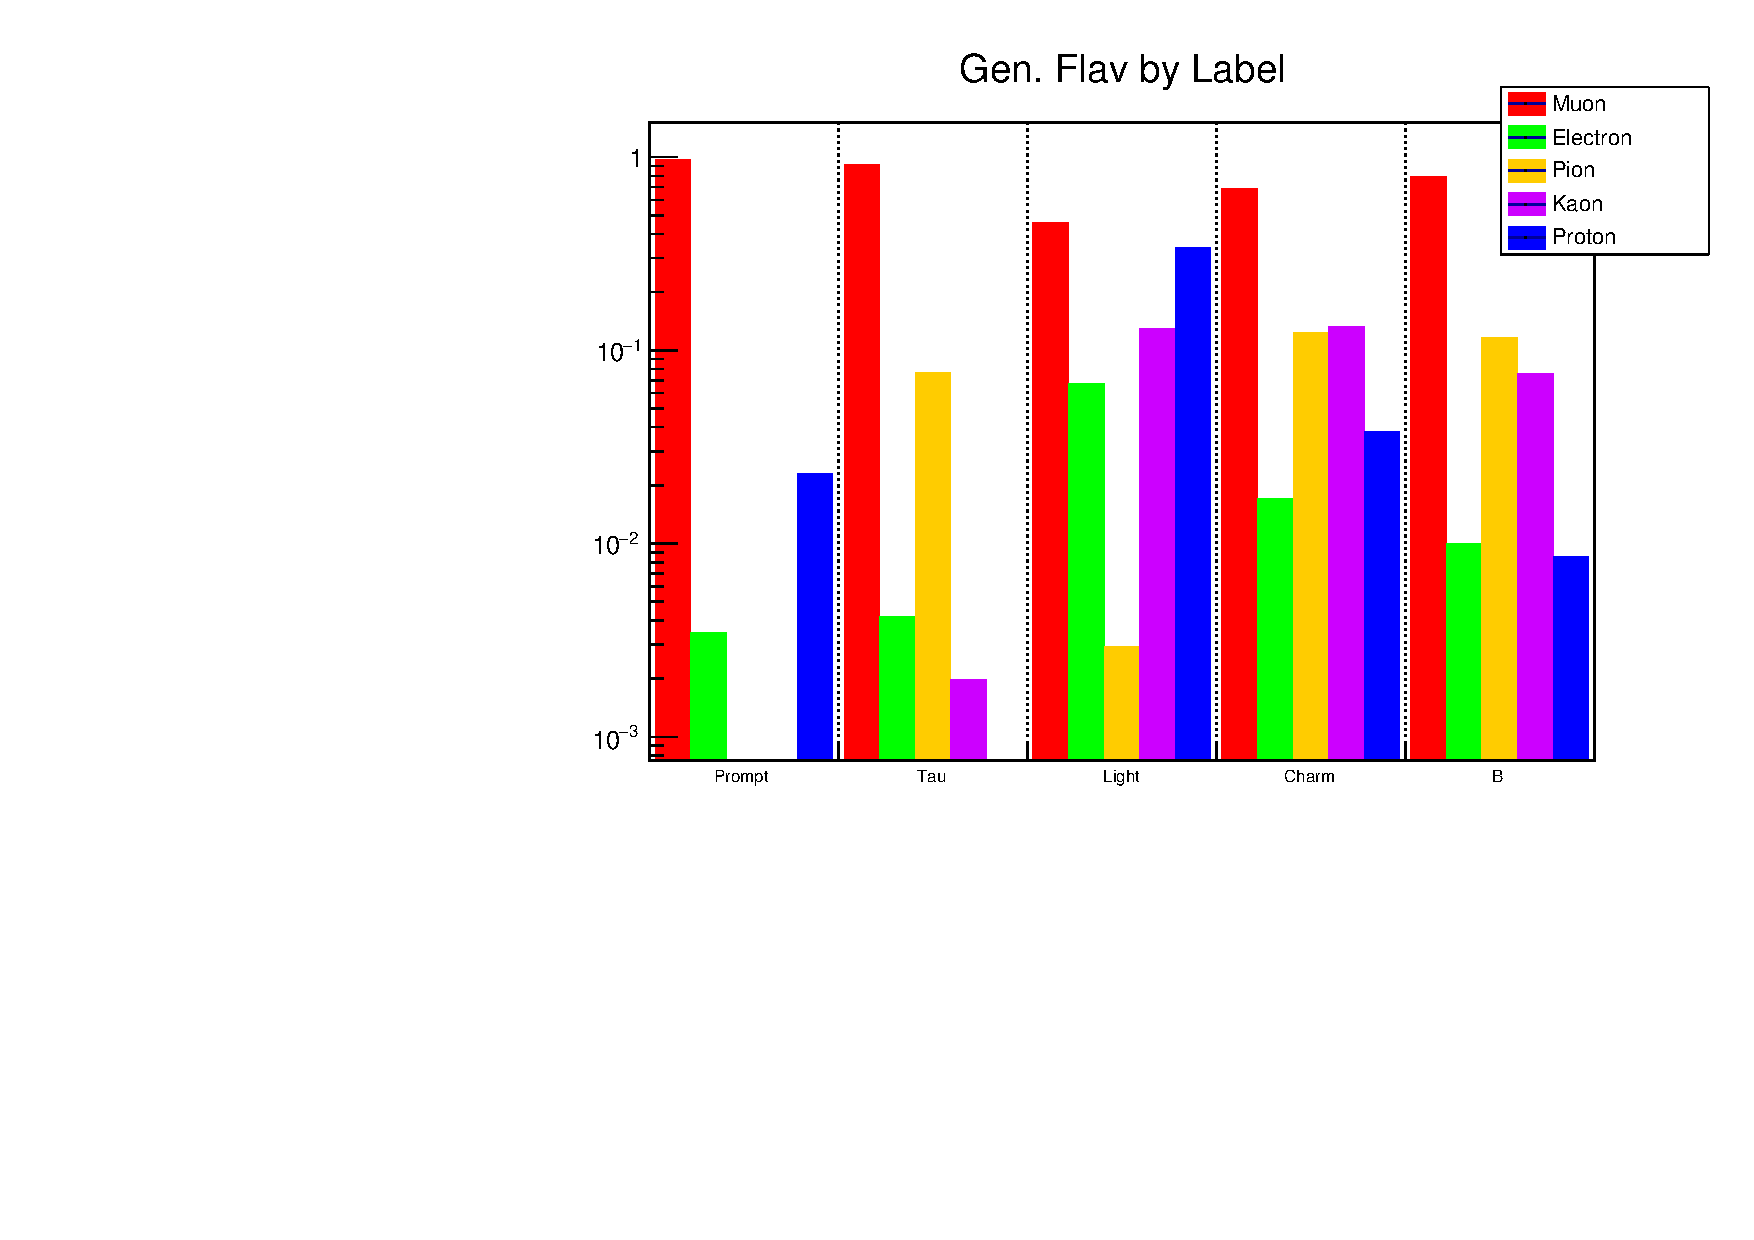
\includegraphics[scale=.3]{tt_flav.pdf}
\end{column}
\end{columns}
\end{frame}


\begin{frame}{ TT } 

\quad \quad \\
\begin{columns}
\begin{column}{0.5\textwidth}

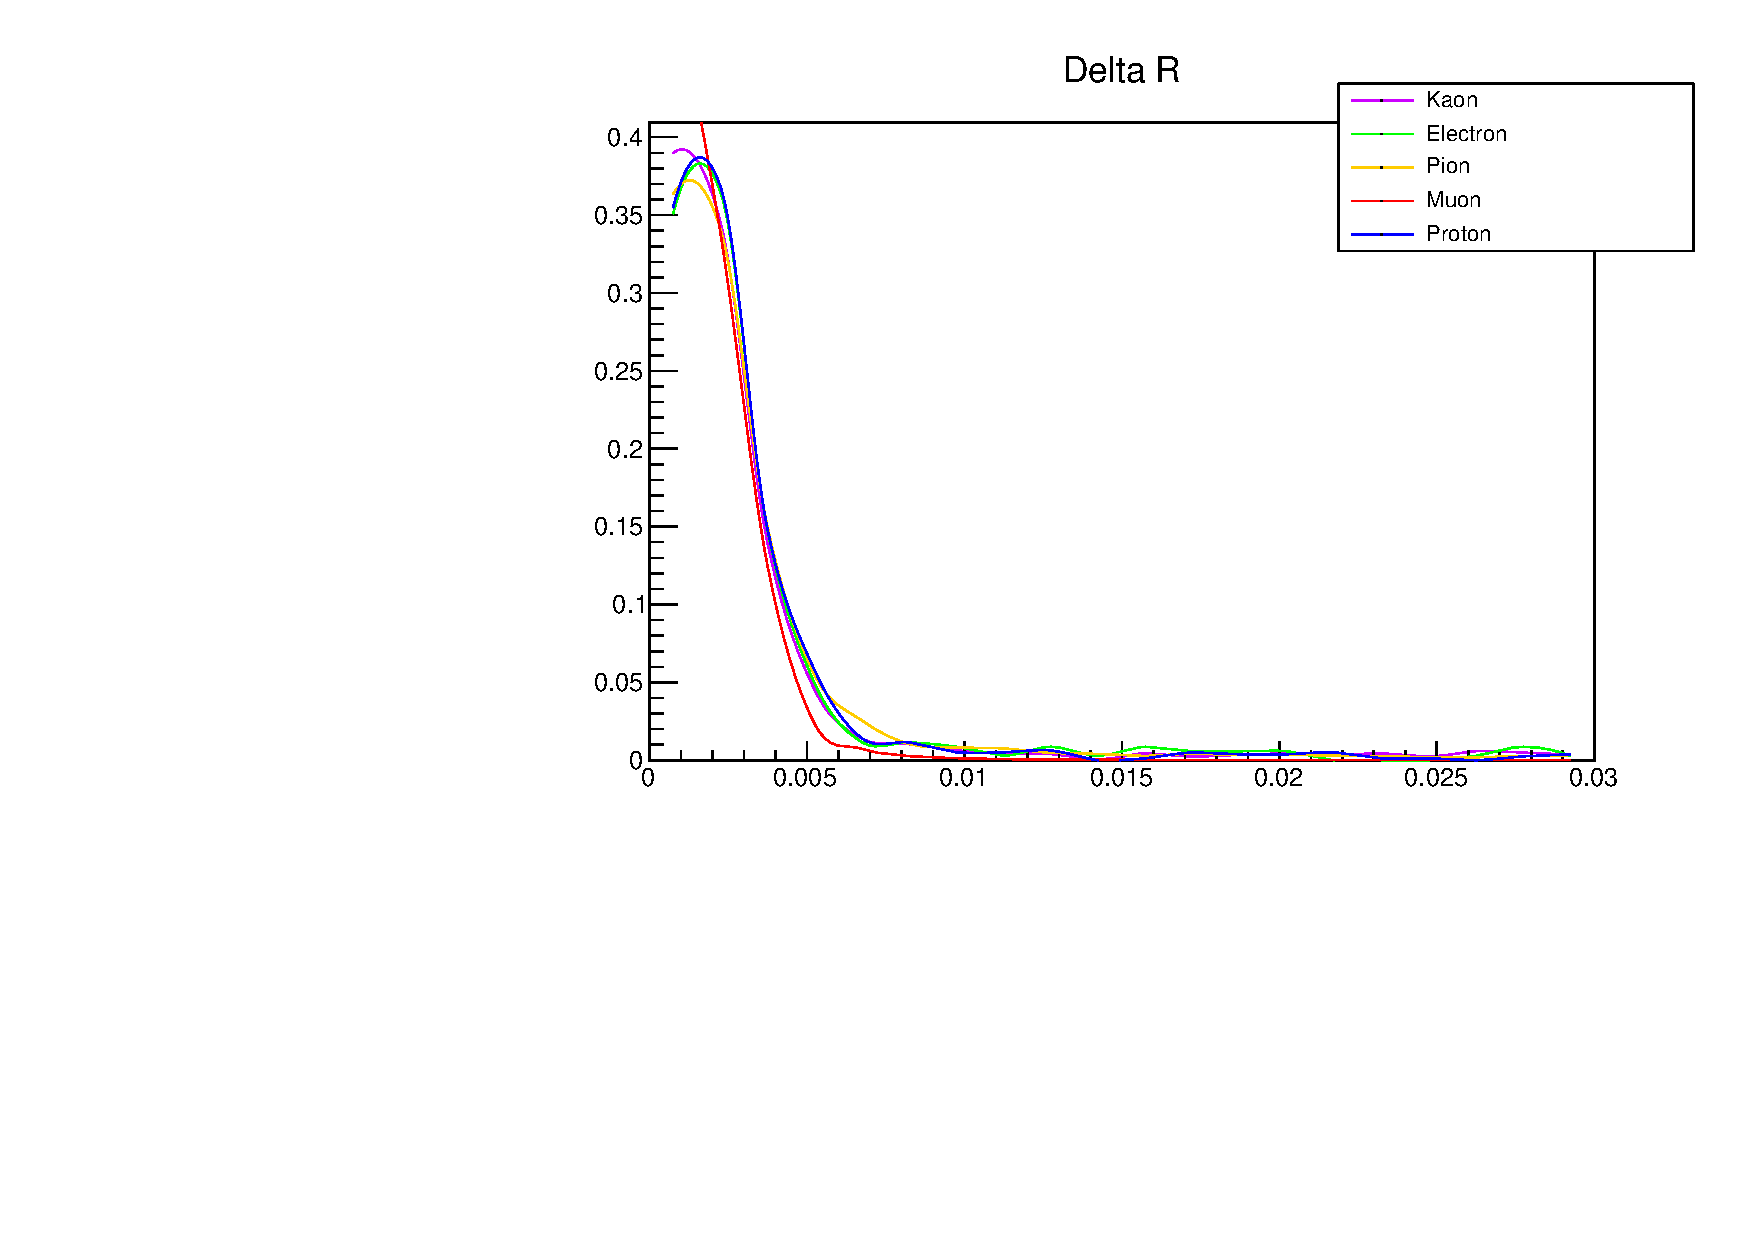
\includegraphics[scale=.3]{tt_dr.pdf}

\end{column}
\begin{column}{0.5\textwidth}

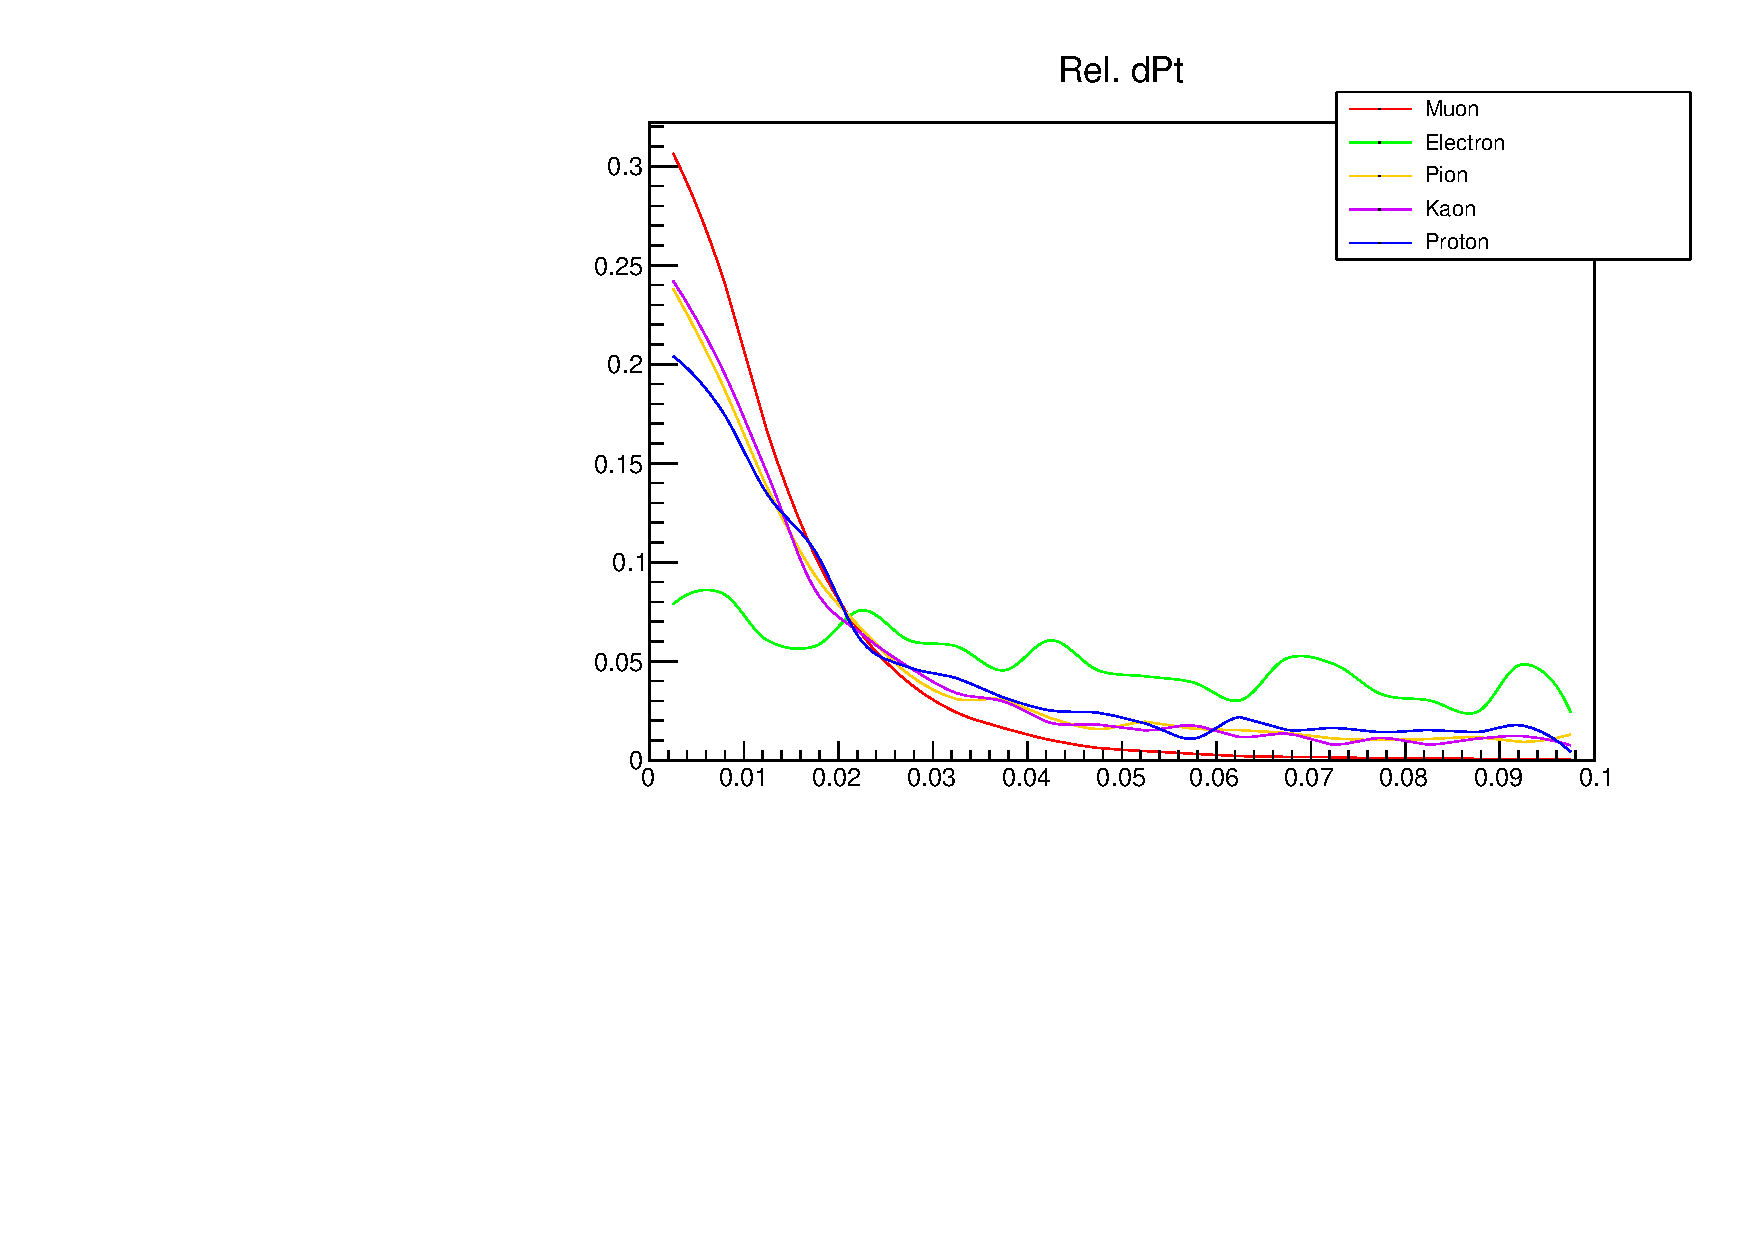
\includegraphics[scale=.3]{tt_dptrel.pdf}
\end{column}
\end{columns}
\end{frame}

%%%%%%%%%%%%%%%%%

\begin{frame}{ QCD } 

\quad \quad \\
\begin{columns}
\begin{column}{0.5\textwidth}
No Cut
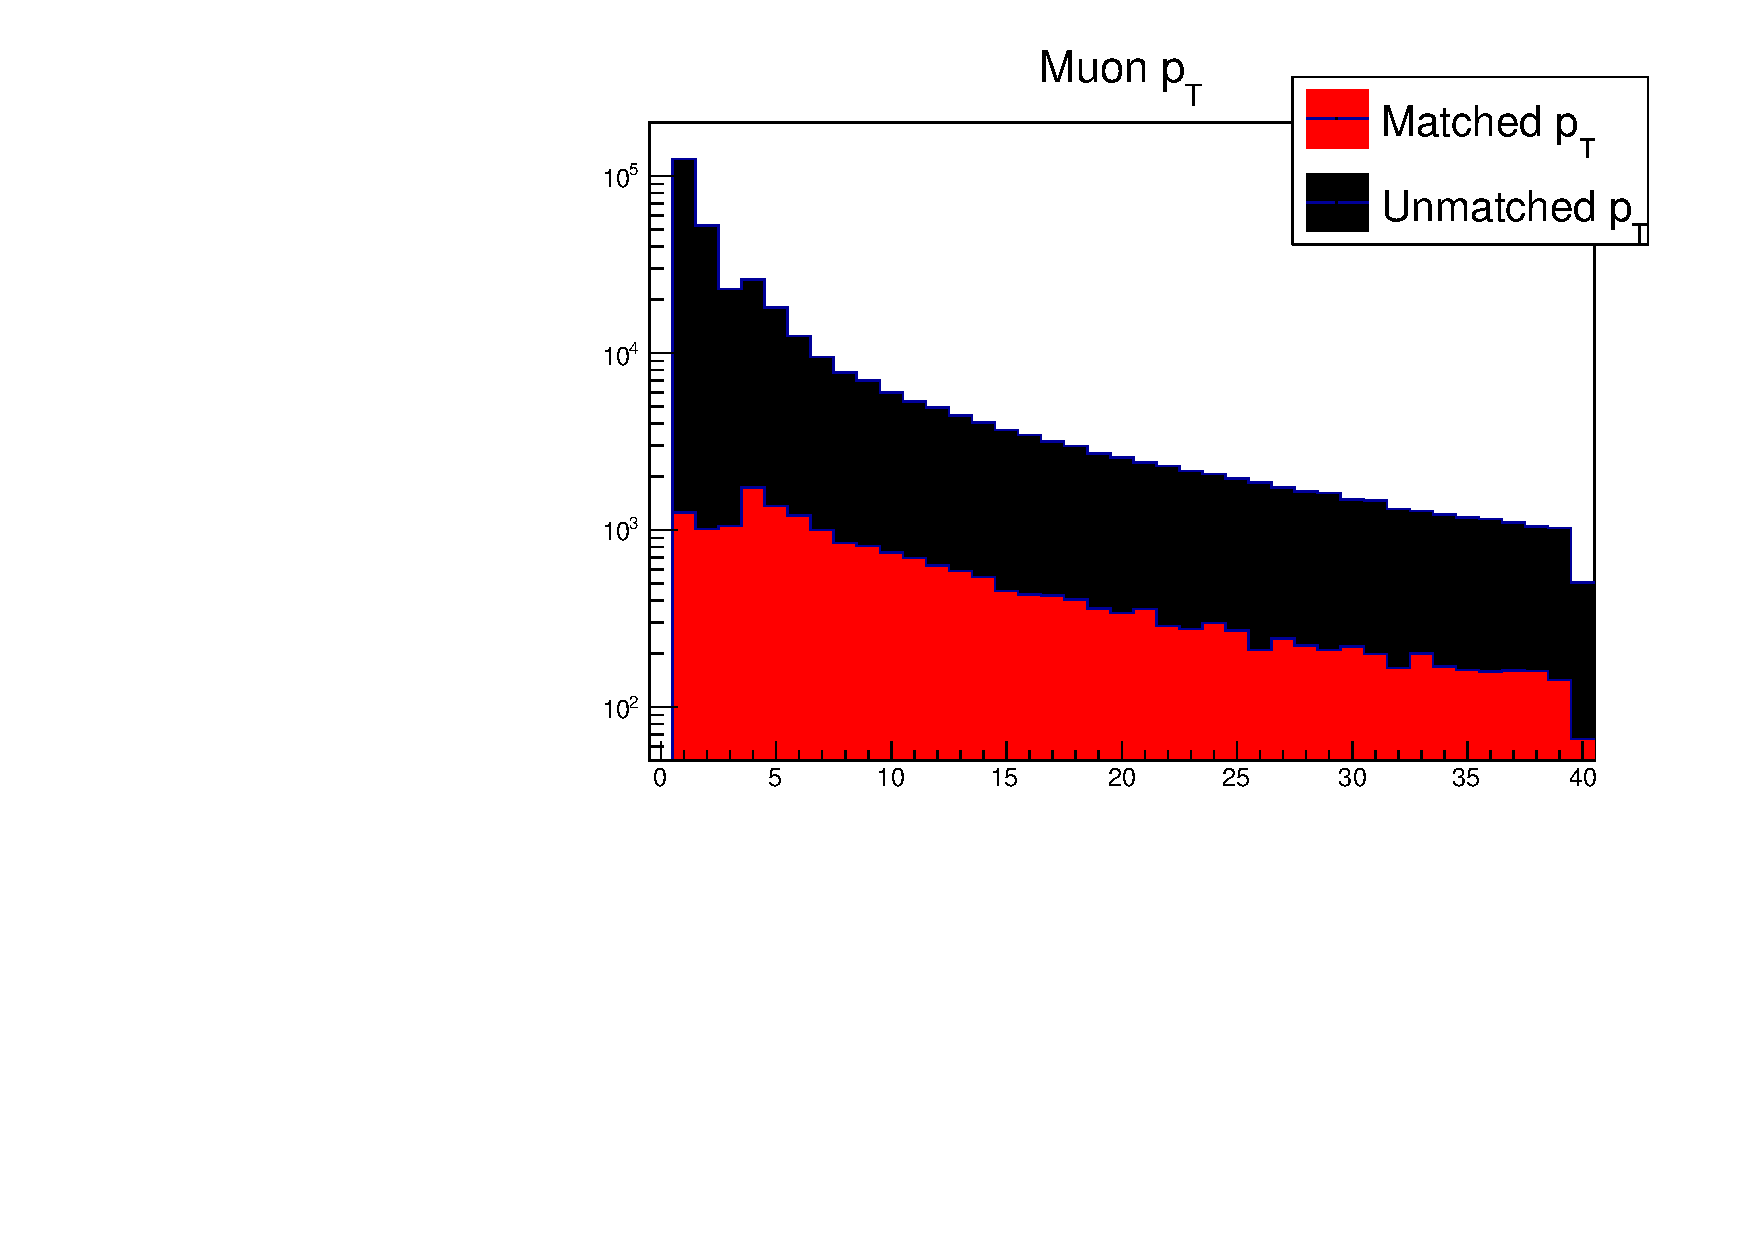
\includegraphics[scale=.3]{qcd_pt.pdf}

\end{column}
\begin{column}{0.5\textwidth}
Reconstructed $p_T > 2 $ GeV
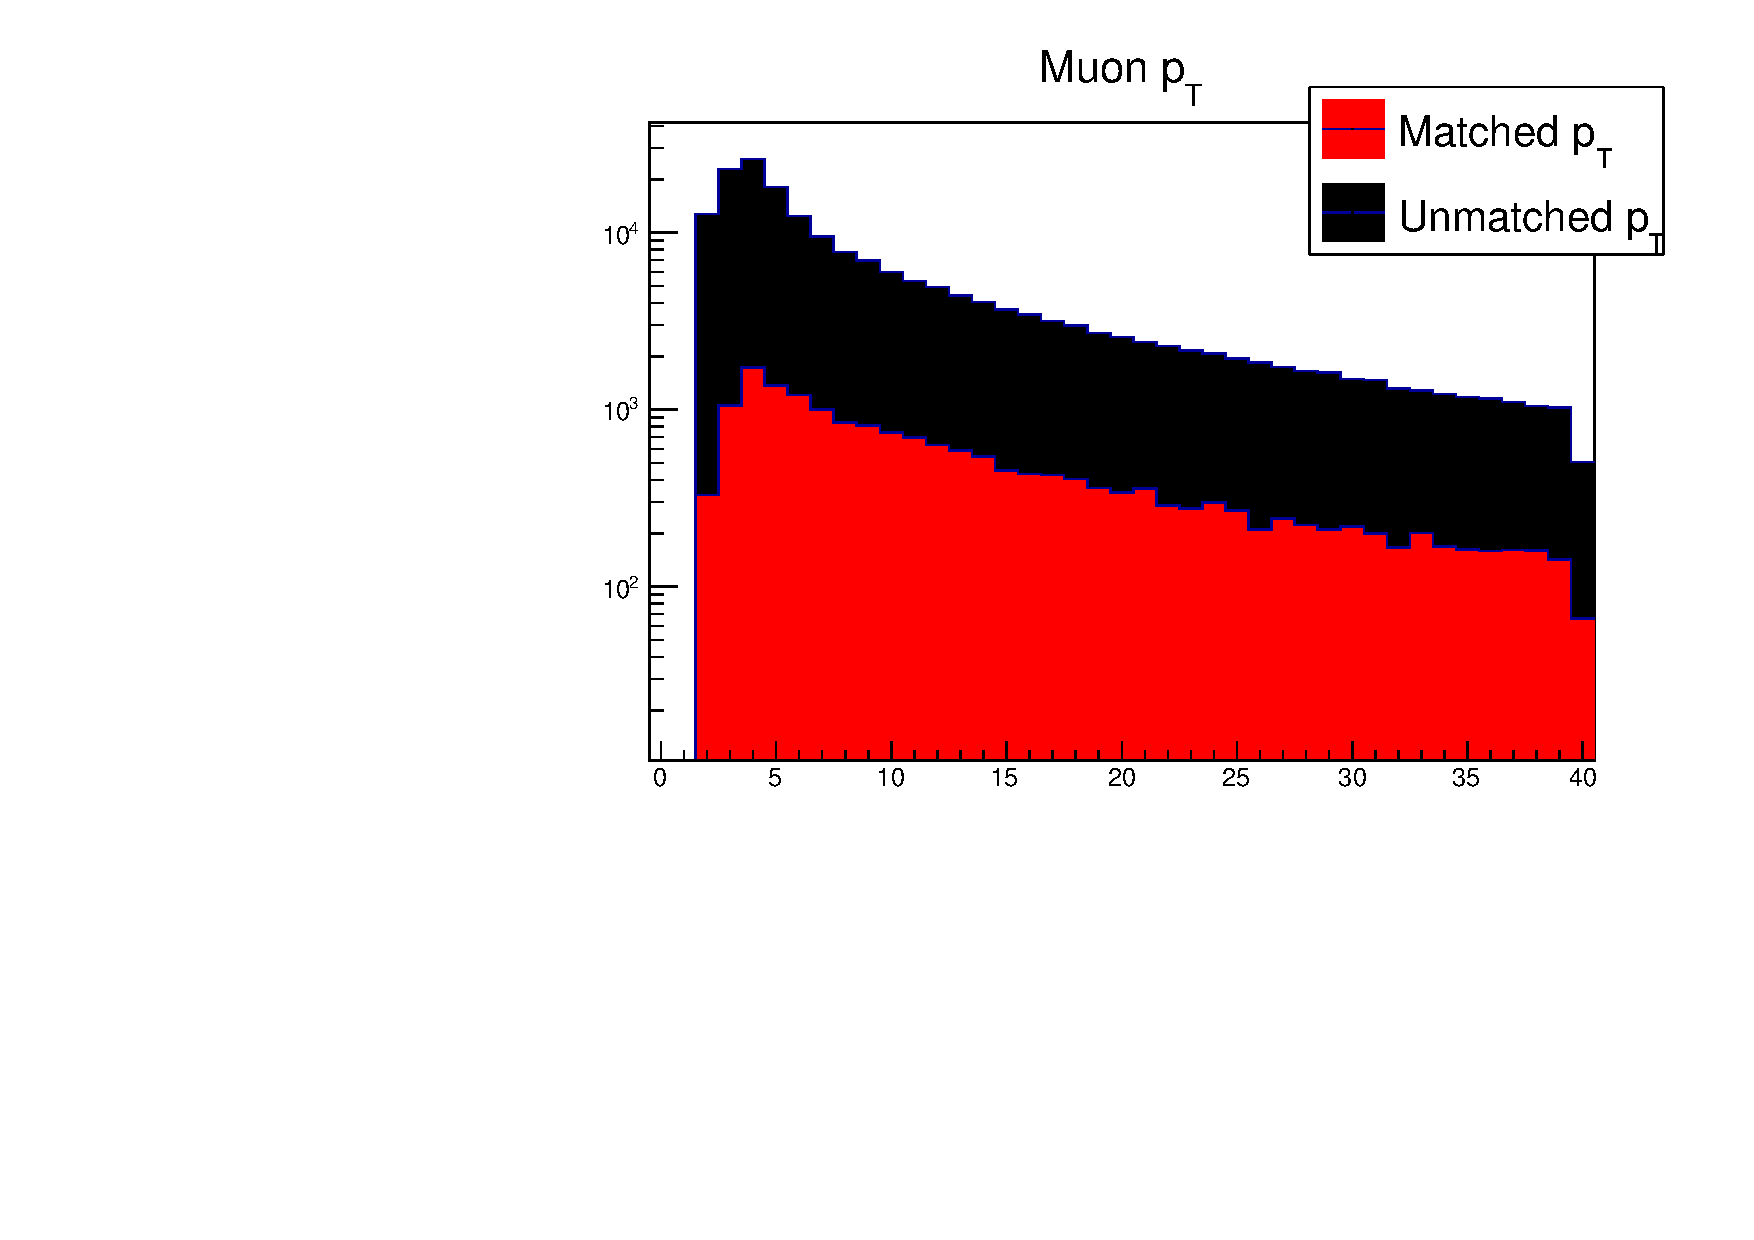
\includegraphics[scale=.3]{qcd_ptcut.pdf}
\end{column}
\end{columns}
\end{frame}



\begin{frame}{ QCD } 

\quad \quad \\
\begin{columns}
\begin{column}{0.5\textwidth}
No Cut
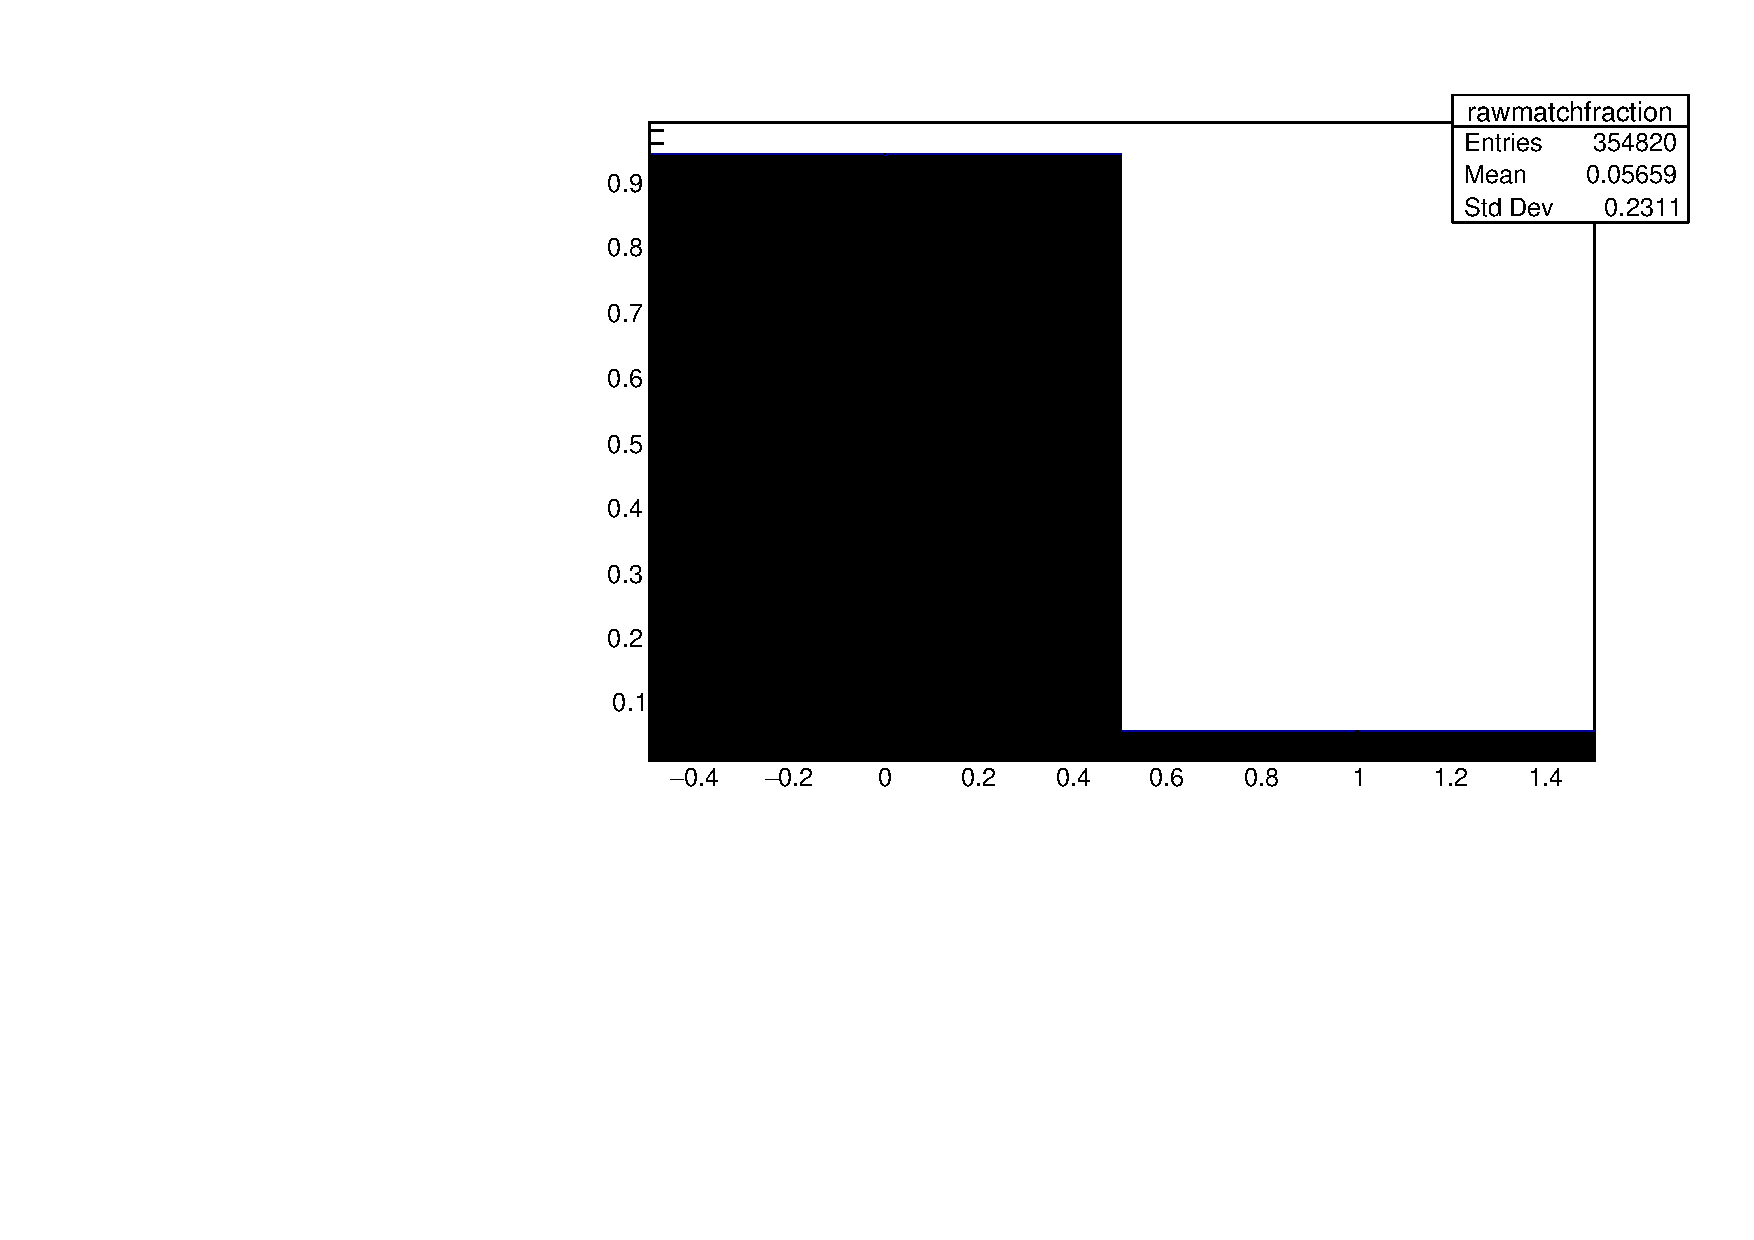
\includegraphics[scale=.3]{qcd_rawmfrac.pdf}

\end{column}
\begin{column}{0.5\textwidth}
Reconstructed $p_T > 2 $ GeV
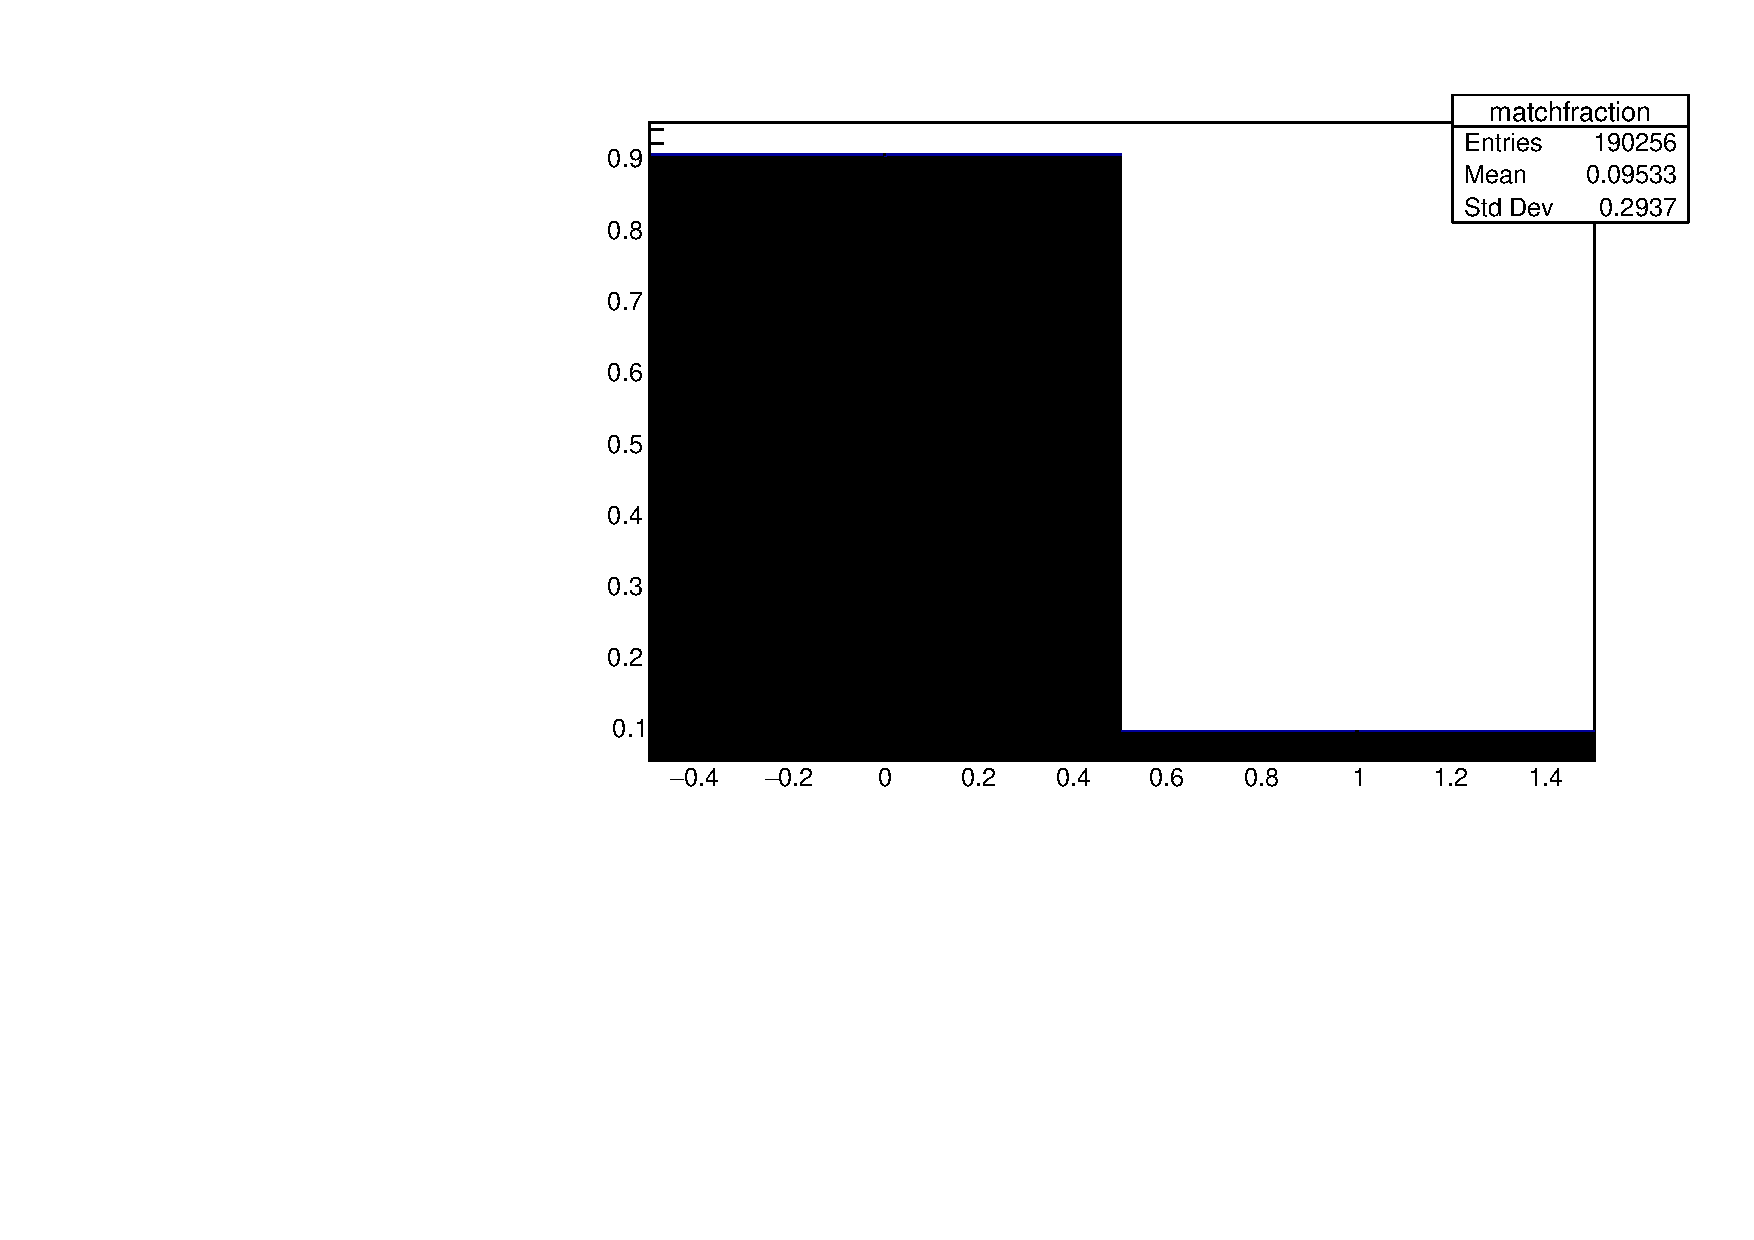
\includegraphics[scale=.3]{qcd_mfrac.pdf}
\end{column}
\end{columns}


\end{frame}


\begin{frame}{ QCD } 

\quad \quad \\
\begin{columns}
\begin{column}{0.5\textwidth}

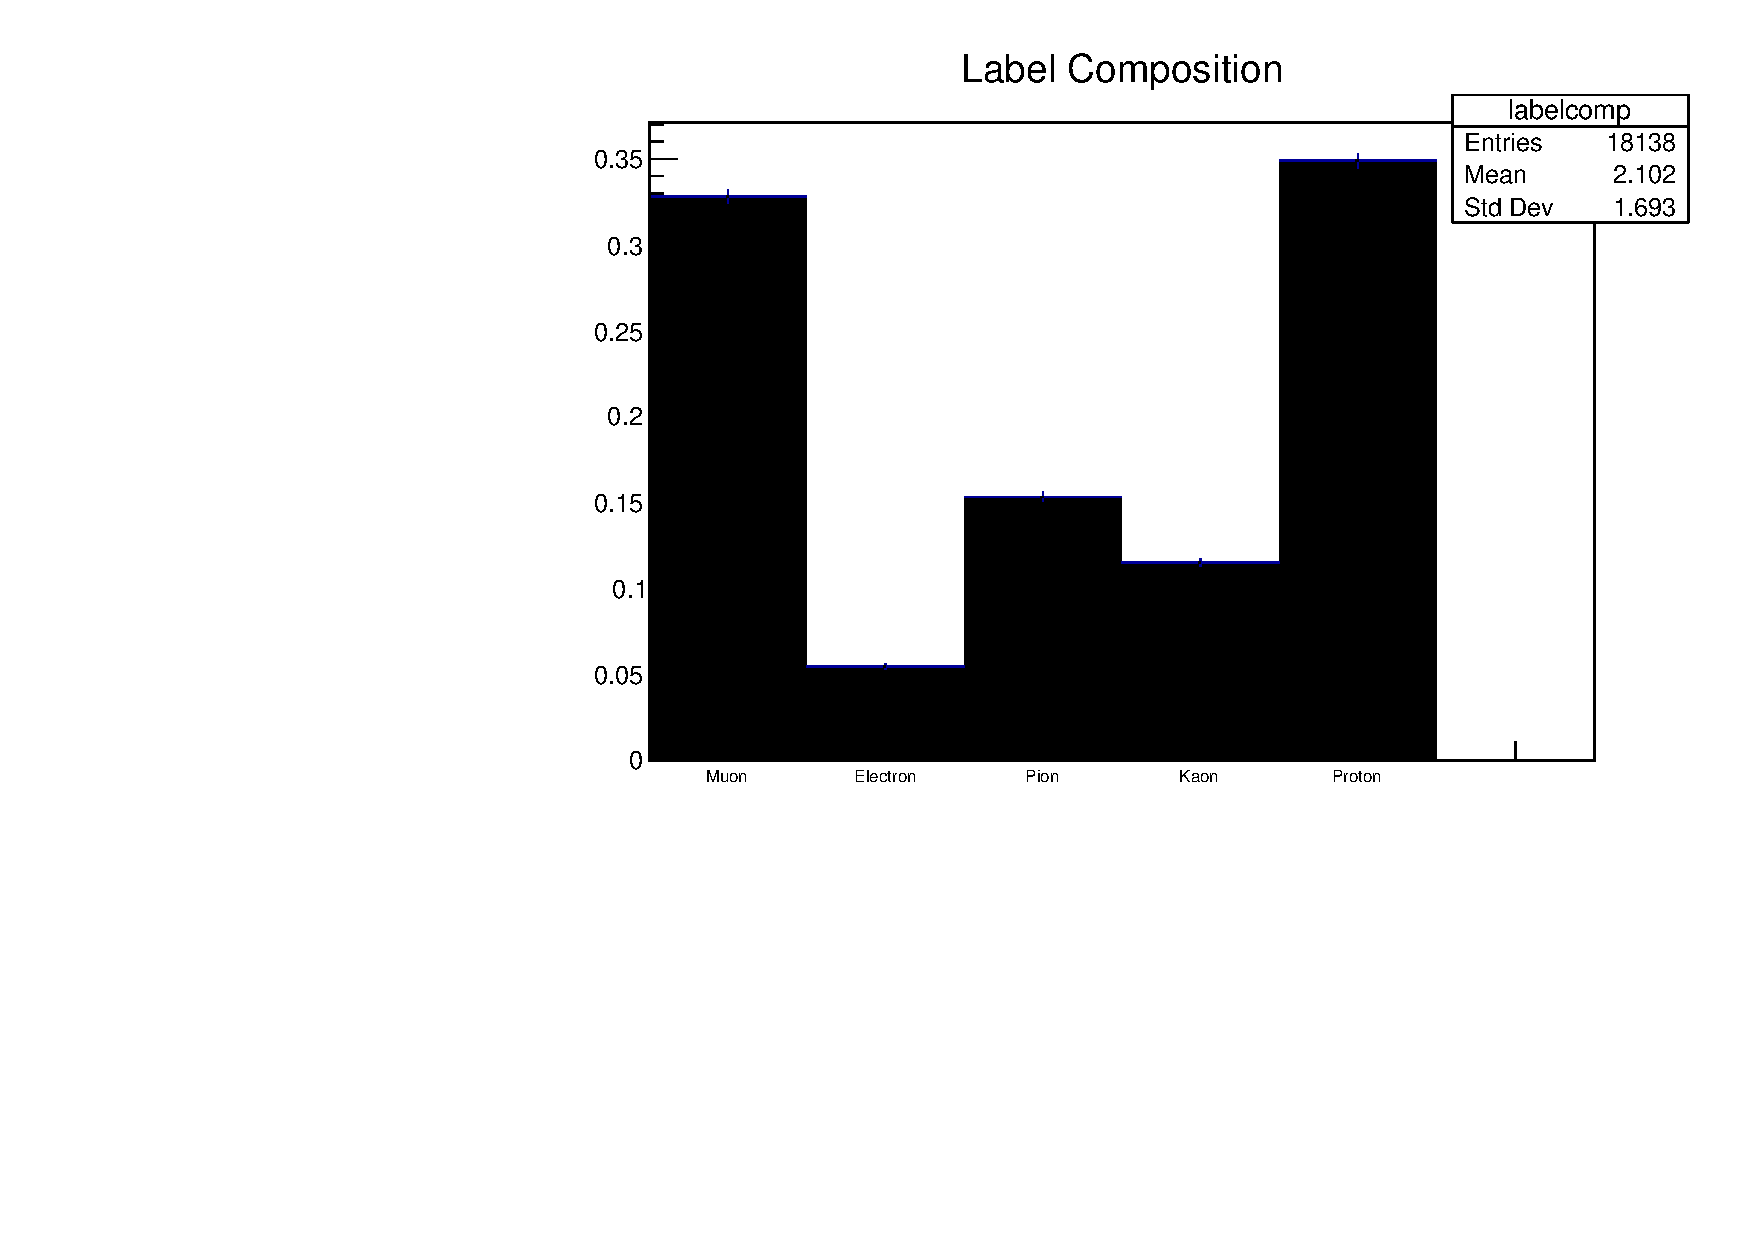
\includegraphics[scale=.3]{qcd_comp.pdf}

\end{column}
\begin{column}{0.5\textwidth}

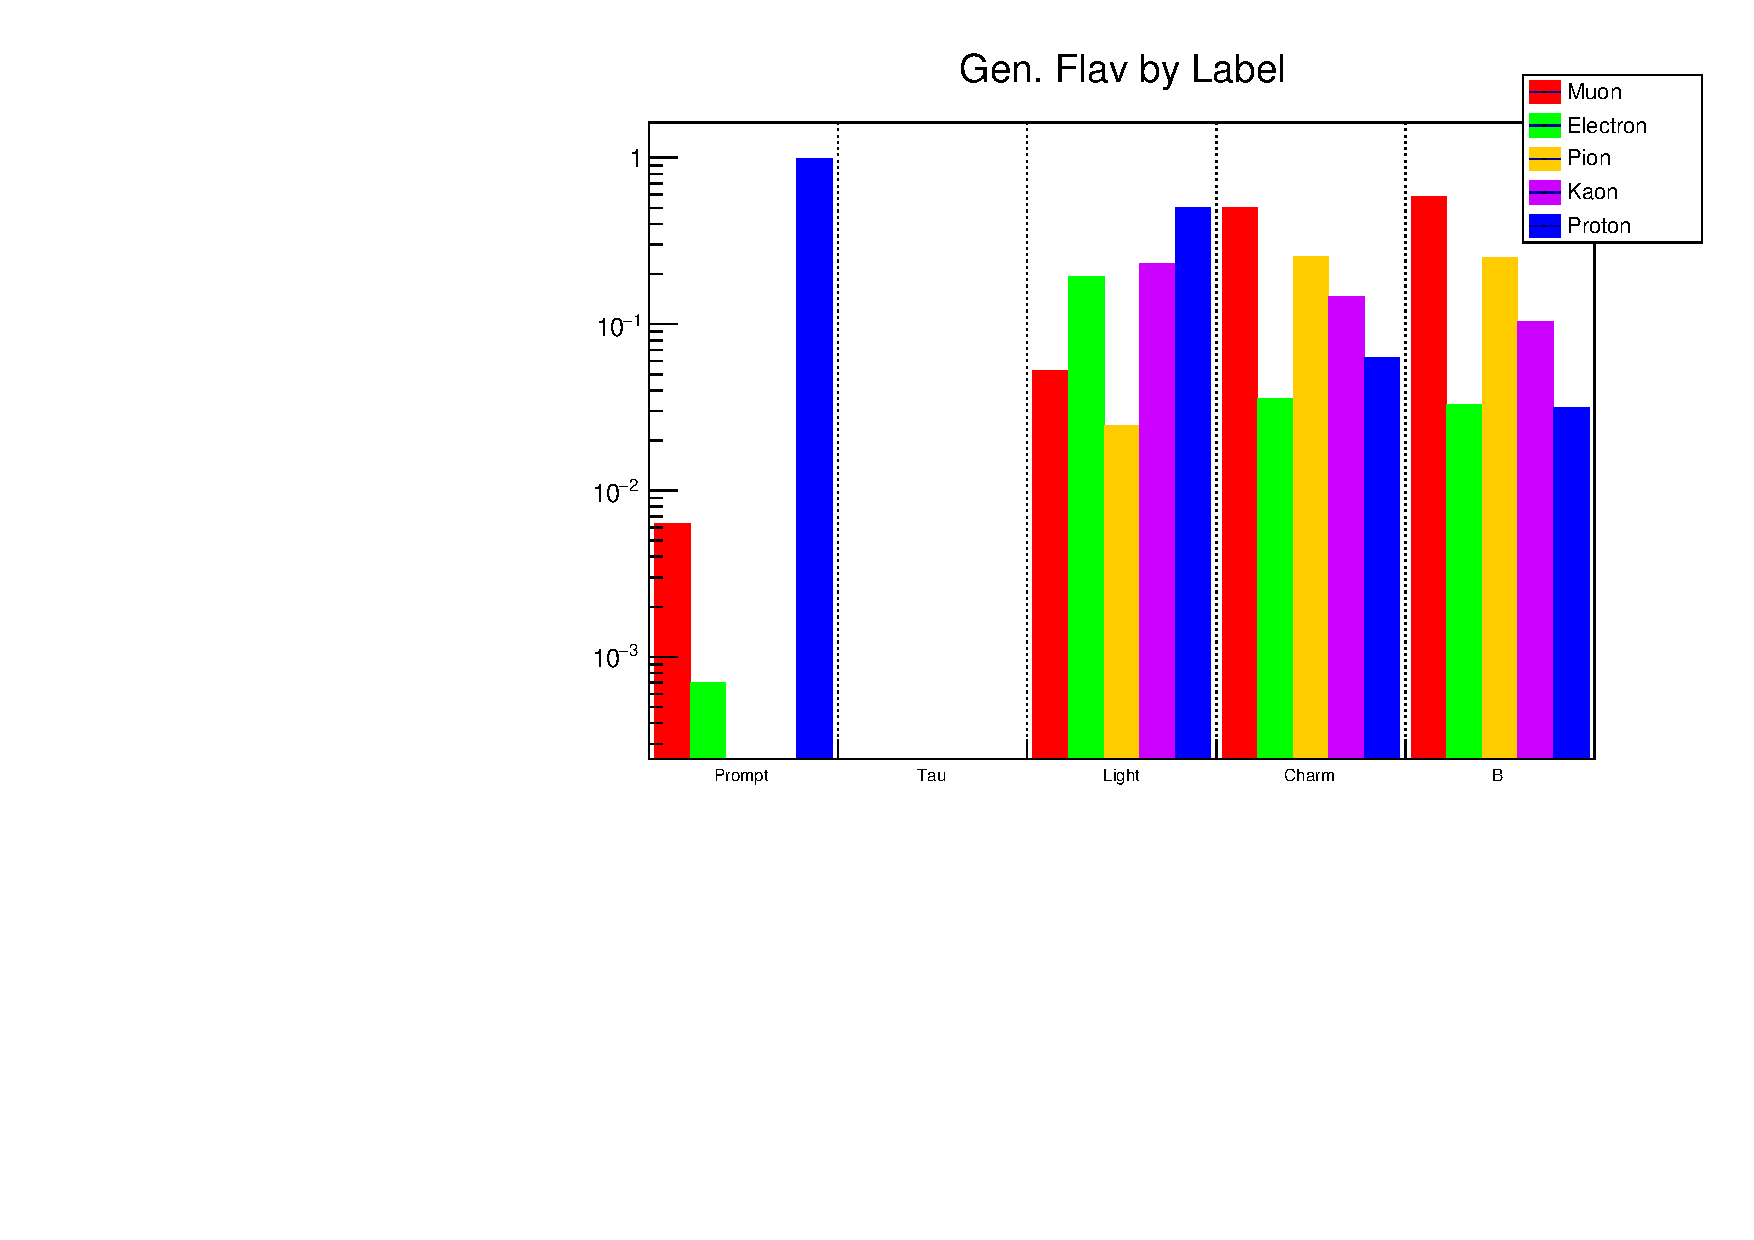
\includegraphics[scale=.3]{qcd_flav.pdf}
\end{column}
\end{columns}
\end{frame}


\begin{frame}{ QCD } 

\quad \quad \\
\begin{columns}
\begin{column}{0.5\textwidth}

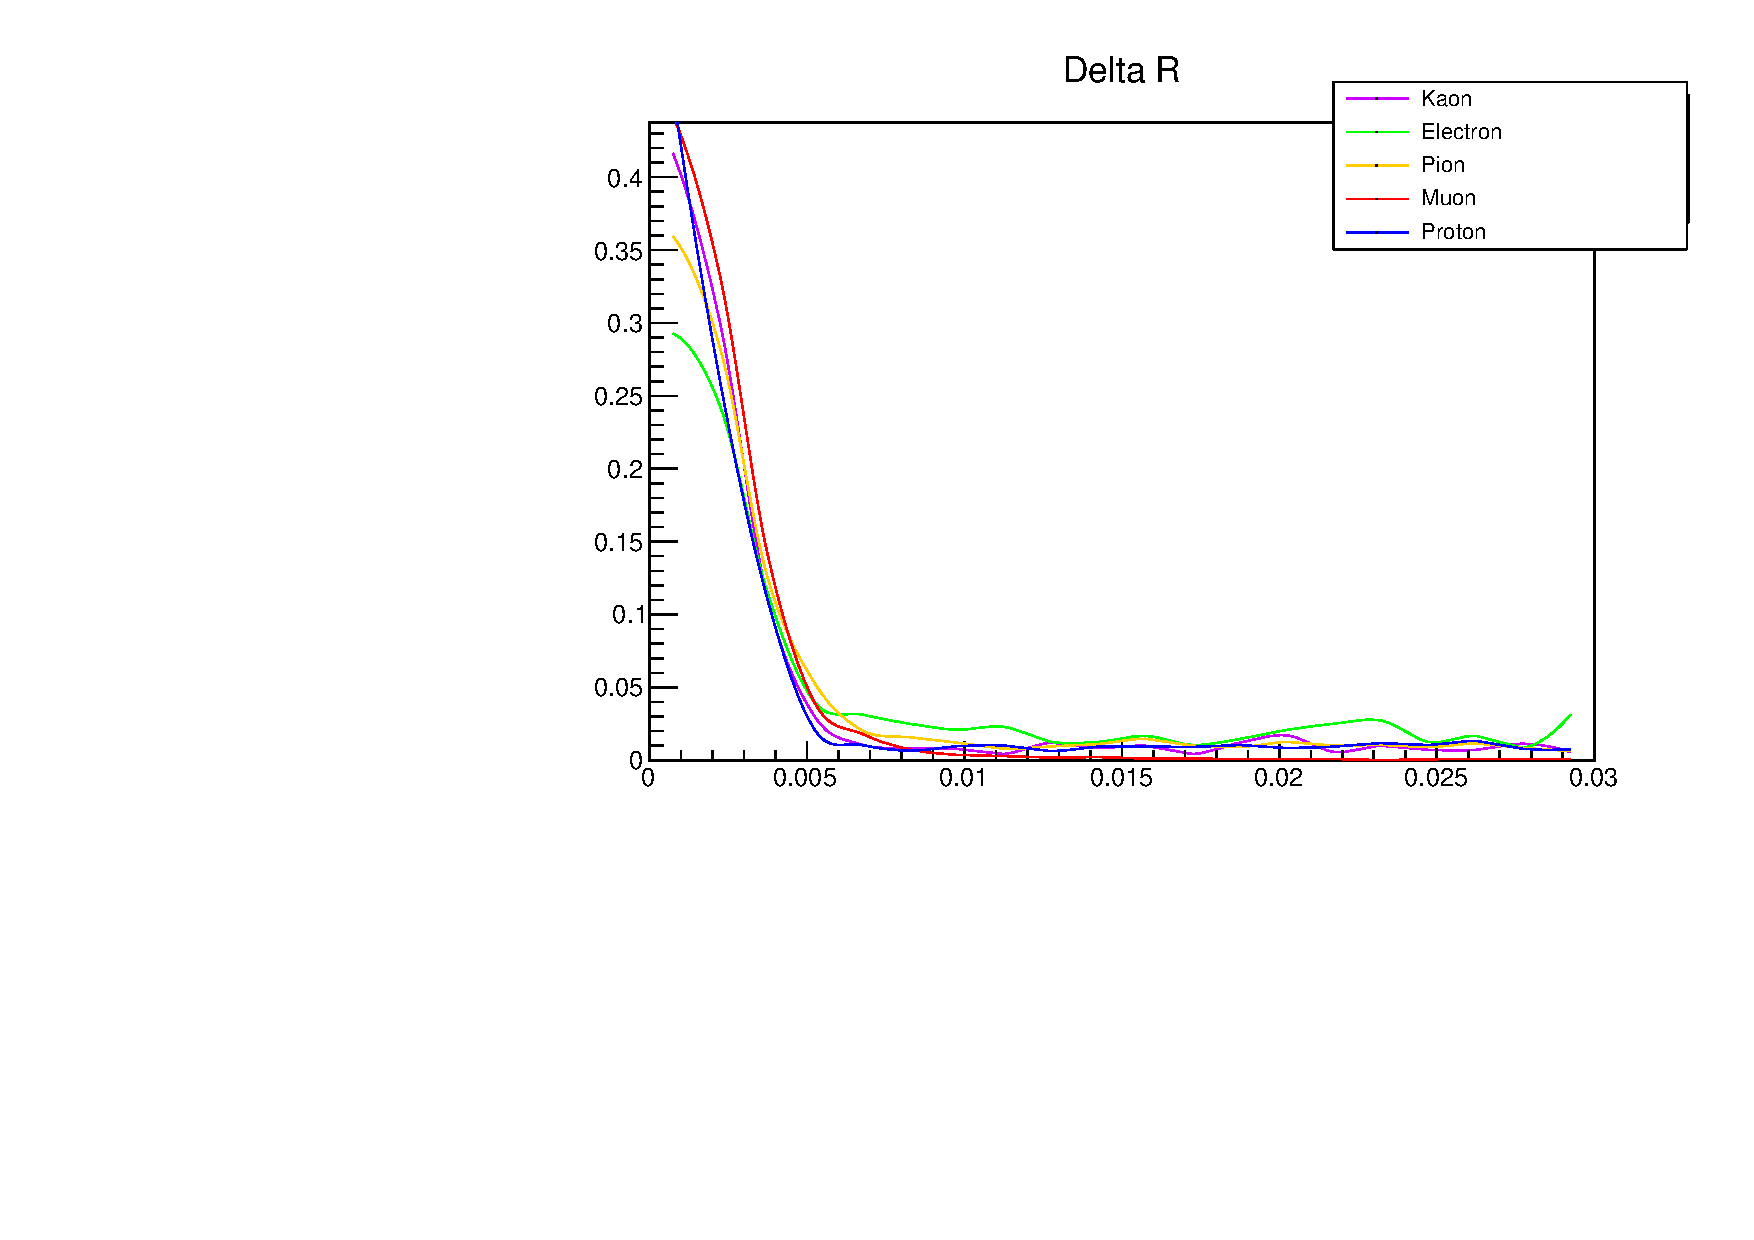
\includegraphics[scale=.3]{qcd_dr.pdf}

\end{column}
\begin{column}{0.5\textwidth}

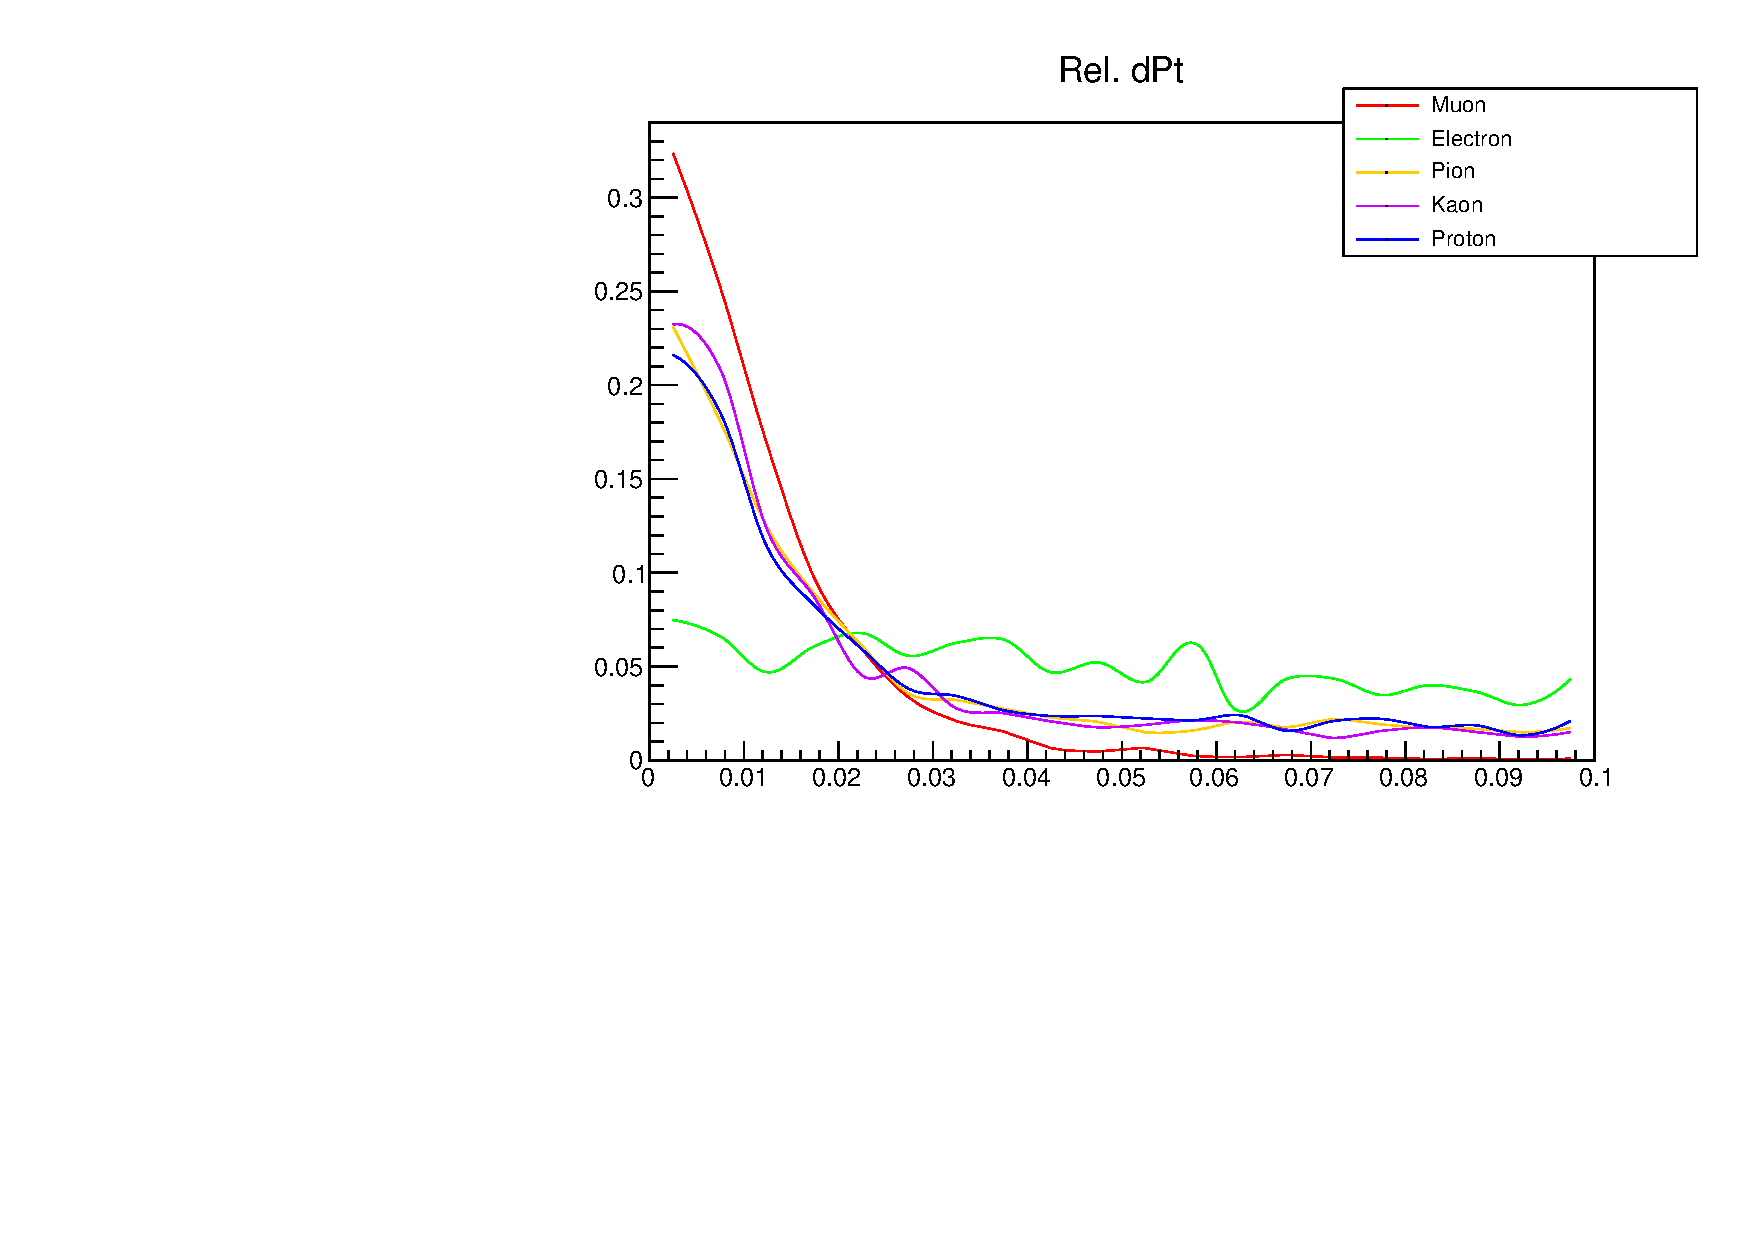
\includegraphics[scale=.3]{qcd_dptrel.pdf}
\end{column}
\end{columns}
\end{frame}


\end{document}